% Options for packages loaded elsewhere
\PassOptionsToPackage{unicode}{hyperref}
\PassOptionsToPackage{hyphens}{url}
\PassOptionsToPackage{dvipsnames,svgnames*,x11names*}{xcolor}
%
\documentclass[
  10pt,
]{article}
\usepackage{lmodern}
\usepackage{amssymb,amsmath}
\usepackage{ifxetex,ifluatex}
\ifnum 0\ifxetex 1\fi\ifluatex 1\fi=0 % if pdftex
  \usepackage[T1]{fontenc}
  \usepackage[utf8]{inputenc}
  \usepackage{textcomp} % provide euro and other symbols
\else % if luatex or xetex
  \usepackage{unicode-math}
  \defaultfontfeatures{Scale=MatchLowercase}
  \defaultfontfeatures[\rmfamily]{Ligatures=TeX,Scale=1}
\fi
% Use upquote if available, for straight quotes in verbatim environments
\IfFileExists{upquote.sty}{\usepackage{upquote}}{}
\IfFileExists{microtype.sty}{% use microtype if available
  \usepackage[]{microtype}
  \UseMicrotypeSet[protrusion]{basicmath} % disable protrusion for tt fonts
}{}
\makeatletter
\@ifundefined{KOMAClassName}{% if non-KOMA class
  \IfFileExists{parskip.sty}{%
    \usepackage{parskip}
  }{% else
    \setlength{\parindent}{0pt}
    \setlength{\parskip}{6pt plus 2pt minus 1pt}}
}{% if KOMA class
  \KOMAoptions{parskip=half}}
\makeatother
\usepackage{xcolor}
\IfFileExists{xurl.sty}{\usepackage{xurl}}{} % add URL line breaks if available
\IfFileExists{bookmark.sty}{\usepackage{bookmark}}{\usepackage{hyperref}}
\hypersetup{
  colorlinks=true,
  linkcolor=Maroon,
  filecolor=Maroon,
  citecolor=Blue,
  urlcolor=blue,
  pdfcreator={LaTeX via pandoc}}
\urlstyle{same} % disable monospaced font for URLs
\usepackage[left=2cm, right=2cm, top=2cm, bottom=3cm, footskip = .5cm]{geometry}
\usepackage{graphicx,grffile}
\makeatletter
\def\maxwidth{\ifdim\Gin@nat@width>\linewidth\linewidth\else\Gin@nat@width\fi}
\def\maxheight{\ifdim\Gin@nat@height>\textheight\textheight\else\Gin@nat@height\fi}
\makeatother
% Scale images if necessary, so that they will not overflow the page
% margins by default, and it is still possible to overwrite the defaults
% using explicit options in \includegraphics[width, height, ...]{}
\setkeys{Gin}{width=\maxwidth,height=\maxheight,keepaspectratio}
% Set default figure placement to htbp
\makeatletter
\def\fps@figure{htbp}
\makeatother
\setlength{\emergencystretch}{3em} % prevent overfull lines
\providecommand{\tightlist}{%
  \setlength{\itemsep}{0pt}\setlength{\parskip}{0pt}}
\setcounter{secnumdepth}{-\maxdimen} % remove section numbering
% Set up the fonts
\usepackage[urw-palatino]{mathdesign}
\usepackage[T1]{fontenc}


% Set the language for 508
\hypersetup{
  pdftitle = {title},
  pdflang = en-US}

% Add accessibility support from http://www.richschwinn.com/accessibility
\RequirePackage{accsupp}
\RequirePackage{pdfcomment}
\newcommand{\AccTool}[2]{\BeginAccSupp{method=pdfstringdef,unicode,Alt={{#1}}}\pdftooltip{{#2}}{{#1}}\EndAccSupp{}}


% Set up the headers and footers
\usepackage{graphicx}
\usepackage{fancyhdr}
\usepackage{ifthen}
\usepackage{everypage}
\usepackage{float}
\usepackage{subfig}

% Avoid struggling over figure and table float in Rmarkdown
\let\origfigure\figure
\let\endorigfigure\endfigure
\renewenvironment{figure}[1][2] {
    \expandafter\origfigure\expandafter[H]
} {
    \endorigfigure
}

\let\origtable\table
\let\endorigtable\endtable
\renewenvironment{table}[1][2] {
    \expandafter\origtable\expandafter[H]
} {
    \endorigtable
}

% First page has the large title and NOAA logo
\pagestyle{fancy}
\fancyhf{}
\setlength\headheight{40pt}
\cfoot{\thepage}

\AddEverypageHook{%
   \ifthenelse{\value{page}=4}%
     {\rhead{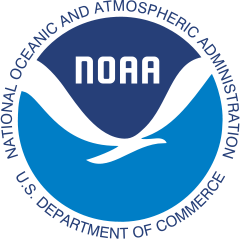
\includegraphics[width=40pt]{images/NOAA_logo.png} \\ \textsf{\emph{March 22, 2021}}}
      \lhead{\textsf{\LARGE State of the Ecosystem 2021: Mid-Atlantic}}
      }%
     {\rhead{}
      \lhead{\textsf{\emph{State of the Ecosystem 2021: Mid-Atlantic}}}
     }
}

\renewcommand{\headrulewidth}{0.4pt}
\renewcommand{\footrulewidth}{0pt}

% Make caption fonts a bit smaller
\usepackage[font={small}]{caption}


% Change section labels to san serif
\usepackage{sectsty}
\allsectionsfont{\normalfont\sffamily\bfseries}
\usepackage{booktabs}
\usepackage{longtable}
\usepackage{array}
\usepackage{multirow}
\usepackage{wrapfig}
\usepackage{float}
\usepackage{colortbl}
\usepackage{pdflscape}
\usepackage{tabu}
\usepackage{threeparttable}
\usepackage{threeparttablex}
\usepackage[normalem]{ulem}
\usepackage{makecell}
\usepackage{xcolor}

\author{}
\date{\vspace{-2.5em}}

\begin{document}

\setcounter{page}{4}

\hypertarget{introduction}{%
\section{Introduction}\label{introduction}}

\hypertarget{about-this-report}{%
\subsection{About This Report}\label{about-this-report}}

This report is for the Mid-Atlantic Fishery Management Council (MAFMC).
The purpose of this report is to synthesize ecosystem information to
better meet fishery management objectives, and to update the MAFMC's
Ecosystem Approach to Fishery Management (EAFM) risk assessment. The
major messages of the report are synthesized on pages 1 and 2, and
synthesis themes are illustrated on page 3. The information in this
report is organized into two sections;
\protect\hyperlink{performance-relative-to-fishery-management-objectives}{performance
measured against ecosystem-level management objectives} (Table
\ref{tab:management-objectives}), and potential
\protect\hyperlink{risks-to-meeting-fishery-management-objectives}{risks
to meeting fishery management objectives}
(\protect\hyperlink{climate-and-ecosystem-productivity}{climate change}
and \protect\hyperlink{other-ocean-uses-offshore-wind}{other ocean
uses}).

\hypertarget{report-structure}{%
\subsection{Report structure}\label{report-structure}}

The two main sections contain subsections for each management objective
or potential risk. Within each subsection, we first review indicator
trends, and the status of the most recent year relative to a threshold
(if available) or relative to the long-term average. Second, we
synthesize results of other indicators and information to outline
potential implications for management (i.e., connecting indicator(s)
status to management and why an indicator(s) is important). For example,
if there are multiple drivers related to an indicator trend, which
drivers may be more or less supported by current information, and which,
if any, can be affected by management action? Similarly, which risk
indicators warrant continued monitoring to evaluate whether regime
shifts or ecosystem reorganization are likely? We emphasize that these
implications are intended to represent testable hypotheses at present,
rather than ``answers,'' because the science behind these indicators and
syntheses continues to develop.

A glossary of terms\footnote{\url{https://noaa-edab.github.io/tech-doc/glossary.html}},
detailed technical methods documentation\footnote{\url{https://NOAA-EDAB.github.io/tech-doc}}
and indicator data\footnote{\url{https://github.com/NOAA-EDAB/ecodata}}
are available online. The details of standard figure formatting (Fig.
\ref{fig:docformat}a), categorization of fish and invertebrate species
into feeding groups (Table \ref{tab:species-groupings}), and definitions
of ecological production units (EPUs, including the Mid-Atlantic Bight,
MAB; Fig. \ref{fig:docformat}b) are provided at the end of the document.

\begin{table}[!h]

\caption{\label{tab:management-objectives}Ecosystem-scale fishery management objectives in the Mid-Atlantic Bight}
\centering
\begin{tabular}[t]{ll}
\toprule
\textbf{Objective Categories} & \textbf{Indicators reported here}\\
\midrule
\addlinespace[0.3em]
\multicolumn{2}{l}{\textbf{Provisioning and Cultural Services}}\\
\hspace{1em}Seafood Production & Landings; commercial total and by feeding guild; recreational harvest\\
\hspace{1em}Profits & Revenue decomposed to price and volume\\
\hspace{1em}Recreation & Days fished; recreational fleet diversity\\
\hspace{1em}Stability & Diversity indices (fishery and ecosystem)\\
\hspace{1em}Social \& Cultural & Community engagement/reliance status\\
\hspace{1em}Protected Species & Bycatch; population (adult and juvenile) numbers, mortalities\\
\addlinespace[0.3em]
\multicolumn{2}{l}{\textbf{Supporting and Regulating Services}}\\
\hspace{1em}Biomass & Biomass or abundance by feeding guild from surveys\\
\hspace{1em}Productivity & Condition and recruitment of managed species, Primary productivity\\
\hspace{1em}Trophic structure & Relative biomass of feeding guilds, Zooplankton\\
\hspace{1em}Habitat & Estuarine and offshore habitat conditions\\
\bottomrule
\end{tabular}
\end{table}

\hypertarget{performance-relative-to-fishery-management-objectives}{%
\section{Performance relative to fishery management
objectives}\label{performance-relative-to-fishery-management-objectives}}

In this section, we examine indicators related to broad, ecosystem-level
fishery management objectives. We also provide hypotheses on the
implications of these trends---\emph{why} we are seeing them, what's
driving them, and potential or observed regime shifts or changes in
ecosystem structure. Identifying multiple drivers, regime shifts, and
potential changes to ecosystem structure, as well as identifying the
most vulnerable resources, can help managers determine whether we can do
anything differently to meet objectives and how to prioritize for
upcoming issues/risks.

\hypertarget{seafood-production}{%
\subsection{Seafood Production}\label{seafood-production}}

\hypertarget{indicators-landings-total-and-by-feeding-guild}{%
\subsubsection{Indicators: Landings; total and by feeding
guild}\label{indicators-landings-total-and-by-feeding-guild}}

All seafood landed by commercial fisheries (total landings) and MAFMC's
managed species landings (a subset of the total) continue to trend
downward in the MAB (Fig. \ref{fig:total-landings}). The downward trend
is most significant in the benthos (clams) group (Fig.
\ref{fig:comm-landings}).

\begin{figure}

{\centering \includegraphics{SOE-MAFMC-2021_files/figure-latex/total-landings-1} 

}

\caption{Total commercial seafood landings (black) and Mid-Atlantic managed seafood landings (red).}\label{fig:total-landings}
\end{figure}

\begin{figure}

{\centering \includegraphics{SOE-MAFMC-2021_files/figure-latex/comm-landings-1} 

}

\caption{Total commercial landings (black) and MAFMC managed species landings (red) by feeding guild.}\label{fig:comm-landings}
\end{figure}

Total recreational harvest (retained fish presumed to be eaten) is also
down in the MAB (Fig. \ref{fig:rec-landings}).

\begin{figure}

{\centering \includegraphics{SOE-MAFMC-2021_files/figure-latex/rec-landings-1} 

}

\caption{Total recreational seafood harvest (millions of fish) in the Mid-Atlantic region.}\label{fig:rec-landings}
\end{figure}

Recreational shark landings show an increase in pelagic sharks over the
past decade, with a sharp decrease in 2018 and 2019 (Fig
\ref{fig:rec_hms}). This is likely influenced by regulatory changes
implemented in 2018 intended to rebuild shortfin mako stocks.

\begin{figure}

{\centering \includegraphics{SOE-MAFMC-2021_files/figure-latex/rec_hms-1} 

}

\caption{Recreational shark landings from Large Pelagics Survey.}\label{fig:rec_hms}
\end{figure}

Aquaculture production is not yet included in total seafood landings,
but we are working toward including it in future reports. Available
aquaculture production of oysters for a subset of Mid-Atlantic states is
trending upward.\footnote{\url{https://noaa-edab.github.io/ecodata/human_dimensions_MAB\#Commercial};
  ``Oyster Aquaculture'' tab}

\hypertarget{implications}{%
\subsubsection{Implications}\label{implications}}

Declining commercial and recreational landings can be driven by many
interacting factors, including combinations of ecosystem and stock
production, management actions, market conditions, and environmental
change. While we cannot evaluate all possible drivers at present, here
we evaluate the extent to which ecosystem overfishing (total landings
exceeding ecosystem productive capacity), stock status, and system
biomass trends may play a role.

\hypertarget{ecosystem-overfishing-indices}{%
\paragraph{Ecosystem Overfishing
Indices}\label{ecosystem-overfishing-indices}}

Thresholds for ecosystem-level overfishing based on system production
characteristics have been proposed
{[}\protect\hyperlink{ref-link_global_2019}{1}{]}, and are applied here
for the MAB. The proposed ecosystem overfishing thresholds are
calculated based on \emph{total catch} while our preliminary indicators
are based on \emph{commercial landings}. Therefore, our current
indicators are underestimated compared with the proposed thresholds. In
future reports we may be able to include commercial discards and
recreational removals to evaluate total catch.

Based on either the ratio of total landings to total primary production
(Fogarty Index, Fig. \ref{fig:fogarty}), or total landings per unit area
(Ryther Index, Fig. \ref{fig:ryther}), MAB landings are at or below the
proposed thresholds, so ecosystem overfishing is unlikely to be a major
factor driving decreased landings.\\

\begin{figure}

{\centering \includegraphics{SOE-MAFMC-2021_files/figure-latex/fogarty-1} 

}

\caption{Fogarty Index; the ratio of total landings to total primary production in the MAB. Link and Watson (2019) give an optimal range (green shading) of the Fogarty ratio of 0.22 to 0.92 parts per thousand (PPT). Previous work suggested that index values exceeding 1 to 2 PPT (orange shading) led to ecosystem tipping points.}\label{fig:fogarty}
\end{figure}

\begin{figure}

{\centering \includegraphics{SOE-MAFMC-2021_files/figure-latex/ryther-1} 

}

\caption{Ryther index; total landings presented on a unit area basis for the MAB. Theoretical estimates (Link and Watson, 2019) imply the index should range from 0.3 - 1.1 mt per sq km annually (green shading) with a limit of 3 mt per sq km annually, above which tipping points could occur in fished ecosystems (orange shading). Expected system-wide MSYs can be in the range of 1 to 3 mt per sq km (unshaded).}\label{fig:ryther}
\end{figure}

The amount of potential yield we can expect from a marine ecosystem
depends on the amount of production entering at the base of the food
web, primarily in the form of phytoplankton; the pathways this energy
follows to reach harvested species; the efficiency of transfer of energy
at each step in the food web; and the fraction of this production that
is removed by the fisheries. The fraction of production removed by
fisheries has declined since the late 1990s (Fig. \ref{fig:ppr-mab}).
The overall trend is largely driven by the decrease in landings with an
increase in primary production over the same period. Current fisheries
remove a lower proportion of the ecosystem's primary production now than
in the 1970s, when the Fogarty and Ryther indices suggest that ecosystem
overfishing may have occurred.

\begin{figure}

{\centering \includegraphics{SOE-MAFMC-2021_files/figure-latex/ppr-mab-1} 

}

\caption{Primary production required to support MAB commercial landings. Included are the top species accounting for 80\% of the landings in each year, with 15\% transfer efficiency assumed between trophic levels. PPD is total primary production. The solid line is based on satellite-derived PPD and the dashed line is based on primary production reconstructed using the mean of satellite-derived PPD from 1998-2010.}\label{fig:ppr-mab}
\end{figure}

\hypertarget{stock-status}{%
\paragraph{Stock Status}\label{stock-status}}

Single species management objectives of maintaining biomass above
minimum thresholds and fishing mortality below limits are being met for
all but two MAFMC managed species, though the status of six stocks is
unknown (Fig. \ref{fig:stock-status}). Therefore, stock status and
associated management constraints are unlikely to be driving decreased
landings. To better address the role of management in future reports, we
could examine how the total allowable catch (TAC) and the percentage of
the TAC taken for each species has changed through time.

\begin{figure}

{\centering \includegraphics{SOE-MAFMC-2021_files/figure-latex/stock-status-1} 

}

\caption{Summary of single species status for MAFMC and jointly federally managed stocks (Goosefish and Spiny dogfish). Stocks in green are below the biomass threshold (overfished), stocks in orange are above the biomass threshold but below the biomass target, and stocks in purple are above the biomass target. Only one stock, Atlantic mackerel, has fishing mortality above the limit (subject to overfishing).}\label{fig:stock-status}
\end{figure}

\hypertarget{system-biomass}{%
\paragraph{System Biomass}\label{system-biomass}}

Although aggregate biomass trends derived from scientific resource
surveys are mostly stable in the MAB, spring piscivores and fall benthos
show long-term increases (Fig. \ref{fig:nefsc-biomass-mab}). The NEAMAP
Fall 2020 survey was completed and is included here; NEFSC surveys were
not completed in 2020. While managed species make up varying proportions
of aggregate biomass, trends in landings are not mirroring shifts in the
overall trophic structure of survey-sampled fish and invertebrates.
Therefore, major shifts in feeding guilds or ecosystem trophic structure
are unlikely to be driving the decline in landings.

\begin{figure}

{\centering \includegraphics{SOE-MAFMC-2021_files/figure-latex/nefsc-biomass-mab-1} 

}

\caption{Spring (left) and fall (right) surveyed biomass in the Mid-Atlantic Bight. Data from the NEFSC Bottom Trawl Survey are shown in black, with NEAMAP shown in red. The shaded area around each annual mean represents 2 standard deviations from the mean.}\label{fig:nefsc-biomass-mab}
\end{figure}

\hypertarget{effect-on-seafood-production}{%
\paragraph{Effect on Seafood
Production}\label{effect-on-seafood-production}}

Because ecosystem overfishing seems unlikely, stock status is mostly
acceptable, and aggregate biomass trends appear stable, the decline in
commercial landings is most likely driven by market dynamics affecting
the landings of surfclams and ocean quahogs, as landings have been below
quotas for these species.

Climate change also seems to be shifting the distribution of surfclams
and ocean quahogs, resulting in areas with overlapping distributions and
increased mixed landings. Given the regulations governing mixed
landings, this could become problematic in the future and is currently
being evaluated by the Council.

The decline in recreational seafood landings stems from other drivers.
Some of the decline, such as that for recreational shark landings, is
driven by management intended to reduce fishing mortality on mako
sharks. However, NOAA Fisheries' Marine Recreational Information Program
survey methodology was updated in 2018, so it is unclear whether the
record-low landings for species other than sharks in 2018 are driven by
changes in fishing behavior or the change in the survey methodology.

Other environmental changes require monitoring as they may become
important drivers of landings in the future:

\begin{itemize}
\tightlist
\item
  Climate is trending into uncharted territory. Globally, 2020 was tied
  with the warmest year on record\footnote{\url{https://www.nasa.gov/press-release/2020-tied-for-warmest-year-on-record-nasa-analysis-shows}}
  with regional marine heatwaves apparent (see
  \protect\hyperlink{climate-and-ecosystem-productivity}{Climate Risks
  section}).\\
\item
  Stocks are shifting distribution, moving towards the northeast and
  into deeper waters throughout the Northeast US Large Marine Ecosystem
  (Fig. \ref{fig:species-dist}).
\end{itemize}

\begin{figure}

{\centering \includegraphics{SOE-MAFMC-2021_files/figure-latex/species-dist-1} 

}

\caption{Aggregate species distribution metrics for species in the Northeast Large Marine Ecosystem.}\label{fig:species-dist}
\end{figure}

\begin{itemize}
\tightlist
\item
  Some ecosystem composition and production changes have been observed
  (see \protect\hyperlink{stability}{Stability section}).
\item
  Fishing engagement has declined in some communities (see
  \protect\hyperlink{social-vulnerability}{Social Vulnerability
  section}).
\end{itemize}

\hypertarget{commercial-profits}{%
\subsection{Commercial Profits}\label{commercial-profits}}

\hypertarget{indicators-revenue-a-proxy-for-profits-with-price-and-volume-components}{%
\subsubsection{Indicators: revenue (a proxy for profits), with price and
volume
components}\label{indicators-revenue-a-proxy-for-profits-with-price-and-volume-components}}

Total commercial revenue (black) has increased over the long term, but
the trend may be reversing, with recent total revenue below the
long-term average (Fig. \ref{fig:comm-revenue}). The MAFMC-managed
species revenue (red) has continued its downward trend, with recent
years near a time-series low.

\begin{figure}

{\centering \includegraphics{SOE-MAFMC-2021_files/figure-latex/comm-revenue-1} 

}

\caption{Total revenue for the region (black) and revenue from MAFMC managed species (red).}\label{fig:comm-revenue}
\end{figure}

Revenue earned by harvesting resources is a function of both the
quantity landed of each species and the prices paid for landings. Beyond
monitoring yearly changes in revenue, it is even more valuable to
determine what drives these changes: harvest levels, the mix of species
landed, price changes, or a combination of these. The Bennet Indicator
decomposes revenue change into two parts, one driven by changing
quantities (volumes), and a second driven by changing prices.

Total revenue trends, decomposed to price and volume indicators (Fig.
\ref{fig:bennet}), mirror price and volume indicator trends for the
benthos (clams; orange in Fig. \ref{fig:bennet-all}) group, especially
over the past decade.

\begin{figure}

{\centering \includegraphics{SOE-MAFMC-2021_files/figure-latex/bennet-1} 

}

\caption{Revenue change from the 2015 values in dollars (black), Price (PI), and Volume Indicators (VI) for commercial landings in the Mid-Atlantic Bight.}\label{fig:bennet}
\end{figure}

\begin{figure}

{\centering \includegraphics{SOE-MAFMC-2021_files/figure-latex/bennet-all-1} 

}

\caption{Total component value in dollars (black) for commercial landings in the Mid-Atlantic Bight.}\label{fig:bennet-all}
\end{figure}

\hypertarget{implications-1}{%
\subsubsection{Implications}\label{implications-1}}

The Bennet indicator demonstrates that increasing total revenue early in
the time series is due to increasing quantities landed, which offset
declining prices. Recent declines in prices contributed to falling
revenue as quantities landed did not increase enough to counteract
declining prices.

Changes in other indicators, particularly those driving landings and
those related to climate change, require monitoring as they may become
important drivers of revenue in the future; for example:

\begin{itemize}
\tightlist
\item
  Surfclams and ocean quahogs are sensitive to warming ocean
  temperatures and ocean acidification.\\
\item
  Acidification levels in surfclam summer habitat are approaching, but
  not yet at, levels affecting surfclam growth (see
  \protect\hyperlink{climate-and-ecosystem-productivity}{Climate Risks
  section}).
\end{itemize}

\hypertarget{recreational-opportunities}{%
\subsection{Recreational
Opportunities}\label{recreational-opportunities}}

\hypertarget{indicators-angler-trips-fleet-diversity}{%
\subsubsection{Indicators: Angler trips, fleet
diversity}\label{indicators-angler-trips-fleet-diversity}}

Recreational effort (angler trips) has no significant long term trend,
with current effort near the long-term average (Fig. \ref{fig:rec-op}).
However, recreational fleet diversity has declined over the long term
(Fig. \ref{fig:rec-div}).

\begin{figure}

{\centering \includegraphics{SOE-MAFMC-2021_files/figure-latex/rec-op-1} 

}

\caption{Recreational effort in the Mid-Atlantic.}\label{fig:rec-op}
\end{figure}

\begin{figure}

{\centering \includegraphics{SOE-MAFMC-2021_files/figure-latex/rec-div-1} 

}

\caption{Recreational fleet effort diversity in the Mid-Atlantic.}\label{fig:rec-div}
\end{figure}

\hypertarget{implications-2}{%
\subsubsection{Implications}\label{implications-2}}

The absence of a long-term trend in recreational effort suggests
relative stability in the overall number of recreational opportunities
in the MAB. However, the decline in recreational fleet diversity
suggests a potentially reduced range of opportunities.

The downward effort diversity trend is driven by party/charter
contraction (from a high of 24\% of angler trips to 7\% currently), and
a shift toward shorebased angling. Effort in private boats remained
stable between 36-37\% of angler trips across the entire series.

Changes in recreational fleet diversity can be considered when managers
seek options to maintain recreational opportunities. Shore anglers will
have access to different species than vessel-based anglers, and when the
same species, typically smaller fish. Many states have developed
shore-based regulations where the minimum size is lower than in other
areas and sectors to maintain opportunities in the shore angling sector.

\hypertarget{stability}{%
\subsection{Stability}\label{stability}}

\hypertarget{indicators-fishery-fleet-and-catch-diversity-ecological-component-diversity}{%
\subsubsection{Indicators: fishery fleet and catch diversity, ecological
component
diversity}\label{indicators-fishery-fleet-and-catch-diversity-ecological-component-diversity}}

While there are many potential metrics of stability, we use diversity
indices as a first check to evaluate overall stability in fisheries and
ecosystems. In general, diversity that remains constant over time
suggests a similar capacity to respond to change over time. A
significant change in diversity over time does not necessarily indicate
a problem or an improvement, but does indicate a need for further
investigation. We examine commercial and recreational fleet and species
catch diversity, and diversity in zooplankton, larval, and adult fish.

\hypertarget{fishery-diversity}{%
\paragraph{Fishery Diversity}\label{fishery-diversity}}

Diversity estimates have been developed for fleets and species landed by
commercial vessels with Mid-Atlantic permits. A fleet is defined here as
the combination of gear type (Scallop Dredge, Other Dredge, Gillnet,
Hand Gear, Longline, Bottom Trawl, Midwater Trawl, Pot, Purse Seine, or
Clam Dredge) and vessel length category (Less than 30 ft, 30 to 50 ft,
50 to 75 feet, 75 ft and above). Commercial fishery fleet count and
fleet diversity have been stable over time in the MAB, with current
values near the long-term average (Fig. \ref{fig:commercial-div}). This
indicates similar commercial fleet composition and species targeting
opportunities over time.

\begin{figure}

{\centering \includegraphics{SOE-MAFMC-2021_files/figure-latex/commercial-div-1} 

}

\caption{Fleet diversity and fleet count in the Mid-Atlantic.}\label{fig:commercial-div}
\end{figure}

Commercial fisheries are relying on fewer species relative to the
mid-90s, but current species revenue diversity has been consistent since
then and is currently near the long term average (Fig.
\ref{fig:commercial-div-species-div}).

\begin{figure}

{\centering \includegraphics{SOE-MAFMC-2021_files/figure-latex/commercial-div-species-div-1} 

}

\caption{Species revenue diversity in the Mid-Atlantic.}\label{fig:commercial-div-species-div}
\end{figure}

As noted \protect\hyperlink{recreational-opportunities}{above}
recreational fleet effort diversity is unstable (declining; Fig.
\ref{fig:rec-div}). However, recreational species catch diversity is
stable and has been at or above the long term average in 7 of the last
10 years (Fig. \ref{fig:recdat-div-catch}).

\begin{figure}

{\centering \includegraphics{SOE-MAFMC-2021_files/figure-latex/recdat-div-catch-1} 

}

\caption{Diversity of recreational catch in the Mid-Atlantic.}\label{fig:recdat-div-catch}
\end{figure}

\hypertarget{ecological-diversity}{%
\paragraph{Ecological Diversity}\label{ecological-diversity}}

Ecological diversity indices show mixed trends. Zooplankton diversity is
increasing in the MAB (Fig. \ref{fig:zoo-diversity}). Adult fish
diversity is measured as the expected number of species in a standard
number of individuals sampled from the NEFSC bottom trawl survey. There
is no vessel correction for this metric, so indices collected aboard the
research vessel Albatross IV (up to 2008) and research vessel Bigelow
(2009-present) are calculated separately. Larval fish and adult fish
diversity indices are stable over time, with current values near the
long-term average (Figs. \ref{fig:ichthyo-diversity}, \ref{fig:exp-n}).

\begin{figure}

{\centering \includegraphics{SOE-MAFMC-2021_files/figure-latex/zoo-diversity-1} 

}

\caption{Zooplankton diversity in the Mid-Atlantic Bight, based on Shannon diversity index.}\label{fig:zoo-diversity}
\end{figure}

\begin{figure}

{\centering \includegraphics{SOE-MAFMC-2021_files/figure-latex/ichthyo-diversity-1} 

}

\caption{Larval fish diversity in the Mid-Atlantic Bight, based on Shannon diversity index.}\label{fig:ichthyo-diversity}
\end{figure}

\begin{figure}

{\centering \includegraphics{SOE-MAFMC-2021_files/figure-latex/exp-n-1} 

}

\caption{Adult fish diversity the Mid-Atlantic Bight, based on expected number of species.}\label{fig:exp-n}
\end{figure}

\hypertarget{implications-3}{%
\subsubsection{Implications}\label{implications-3}}

Fleet diversity indices are used by the MAFMC to evaluate stability
objectives as well as risks to fishery resilience and maintaining equity
in access to fishery resources
{[}\protect\hyperlink{ref-gaichas_implementing_2018}{2}{]}.

Stability in commercial fleet diversity metrics suggests stable capacity
to respond to the current range of fishing opportunities.

Declining recreational fleet effort diversity, as noted
\protect\hyperlink{recreational-opportunities}{above}, indicates that
the party/charter boat sector continues to contract, with shoreside
angling becoming more important, as a percentage of recreational days
fished.

Stability in recreational species catch diversity has been maintained by
a different set of species over time. A recent increase in Atlantic
States Marine Fisheries Commission (ASMFC) and South Atlantic Fishery
Management Council (SAFMC) managed species in recreational catch is
helping to maintain diversity in the same range that MAFMC and New
England Fishery Management Council (NEFMC) species supported in the
1990s.

Ecological diversity indices can provide insight into ecosystem
structure. Changes in ecological diversity over time may indicate
altered ecosystem structure with implications for fishery productivity
and management {[}\protect\hyperlink{ref-friedland_changes_2020}{3}{]}.

Increasing zooplankton diversity is driven by the declining dominance of
the calanoid copepod \emph{Centropages typicus}, with a similar
composition of other zooplankton species.

Stable larval and adult fish diversity indicates the same overall number
and evenness over time, but doesn't rule out species substitutions
(e.g., warm-water replacing cold-water). While larval fish diversity is
near the long-term mean, the dominance of a few warm-water taxa has
increased. Stable but variable larval diversity can indicate interannual
changes in a dominant species.

In the MAB, existing diversity indicators suggest overall stability in
the fisheries and ecosystem components examined. However, declining
recreational fleet diversity suggests a potential loss in the range of
recreational fishing opportunities, and increasing zooplankton diversity
is due to the declining dominance of an important species, suggesting
change in the zooplankton community that warrants continued monitoring
to determine if managed species are affected.

\hypertarget{social-vulnerability}{%
\subsection{Social Vulnerability}\label{social-vulnerability}}

\hypertarget{indicators-social-vulnerability-in-commercial-and-recreational-fishing-communities}{%
\subsubsection{Indicators: Social vulnerability in commercial and
recreational fishing
communities}\label{indicators-social-vulnerability-in-commercial-and-recreational-fishing-communities}}

Social vulnerability measures social factors that shape a community's
ability to adapt to change and does not consider gentrification pressure
(see
\href{https://www.fisheries.noaa.gov/national/socioeconomics/social-indicator-definitions}{detailed
definitions}). Communities that ranked medium-high or above for one or
more of the following indicators: poverty, population composition,
personal disruption, or labor force structure, are highlighted in red.

Commercial fishery engagement measures the number of permits, dealers,
and landings in a community, while reliance expresses these numbers
based on the level of fishing activity relative to the total population
of a community.\\
In 2020, we reported that the number of highly engaged Mid-Atlantic
commercial fishing communities had declined over time, and engagement
scores had also declined in medium-highly engaged communities. Here we
focus on the top ten most engaged, and top ten most reliant commercial
fishing communities and their associated social vulnerability (Fig.
\ref{fig:commercial-engagement}). Barnegat Light and Cape May, NJ, and
Reedville, VA are highly engaged and reliant with medium-high to high
social vulnerability.\\

\begin{figure}

{\centering \includegraphics{SOE-MAFMC-2021_files/figure-latex/commercial-engagement-1} 

}

\caption{Commercial engagement, reliance, and social vulnerability for the top commercial fishing communities in the Mid-Atlantic.}\label{fig:commercial-engagement}
\end{figure}

Recreational fishery engagement measures shore, private vessel, and
for-hire fishing activity while reliance expresses these numbers based
on fishing effort relative to the population of a community. Of the nine
recreational communities that are most engaged and reliant, Avon,
Ocracoke and Hatteras, NC and Barnegat Light and Cape May, NJ scored
medium-high or above for social vulnerability (Fig.
\ref{fig:recreational-engagement}).

Both commercial and recreational fishing are important activities in
Montauk, NY; Barnegat Light, Cape May, and Point Pleasant Beach, NJ; and
Ocracoke and Rodanthe, NC, meaning some of these communities may be
impacted simultaneously by commercial and recreational regulatory
changes. Of these communities, three scored medium-high or above for
social vulnerability.

\begin{figure}

{\centering \includegraphics{SOE-MAFMC-2021_files/figure-latex/recreational-engagement-1} 

}

\caption{Recreational engagement, reliance, and social vulnerability for the top recreational fishing communities in the Mid-Atlantic.}\label{fig:recreational-engagement}
\end{figure}

\hypertarget{implications-4}{%
\subsubsection{Implications}\label{implications-4}}

These plots provide a snapshot of the relationship between social
vulnerability and the most highly engaged and most highly reliant
commercial and recreational fishing communities in the Mid-Atlantic.
Similar plots are used to inform the annual
\href{https://www.pcouncil.org/documents/2020/02/g-1-a-iea-team-report-1.pdf/}{California
Current Ecosystem Status Report}. These communities may be vulnerable to
changes in fishing patterns due to regulations and/or climate change.
When any of these communities are also experiencing social
vulnerability, they may have lower ability to successfully respond to
change. These indicators may also point to communities that are
vulnerable to environmental justice issues. Additional analysis related
to ecosystem shifts and
\href{https://www.ecfr.gov/cgi-bin/retrieveECFR?gp=\&SID=6b0acea089174af8594db02314f26914\&mc=true\&r=SECTION\&n=se50.12.600_1345}{National
Standard 8 of the Magnuson-Stevens Act} is ongoing.

\hypertarget{protected-species}{%
\subsection{Protected Species}\label{protected-species}}

Protected species include marine mammals protected under the Marine
Mammal Protection Act, endangered and threatened species protected under
the Endangered Species Act, and migratory birds protected under the
Migratory Bird Treaty Act. In the Northeast U.S., endangered/threatened
species include Atlantic salmon, Atlantic and shortnose sturgeon, all
sea turtle species, and five baleen whales. Fishery management
objectives for protected species generally focus on reducing threats and
on habitat conservation/restoration. Here we report on the status of
these actions as well as indicating the potential for future
interactions driven by observed and predicted ecosystem changes in the
Northeast U.S. region. Protected species objectives include managing
bycatch to remain below potential biological removal (PBR) thresholds,
recovering endangered populations, and monitoring unusual mortality
events (UMEs).

\hypertarget{indicators-bycatch-population-adult-and-juvenile-numbers-mortalities}{%
\subsubsection{Indicators: bycatch, population (adult and juvenile)
numbers,
mortalities}\label{indicators-bycatch-population-adult-and-juvenile-numbers-mortalities}}

Average indices for both harbor porpoise (Fig. \ref{fig:harborporpoise})
and gray seal bycatch (Fig. \ref{fig:grayseal}) are below current PBR
thresholds, meeting management objectives. However, the 2019 bycatch
estimate for gray seals was highest in the time series.

\begin{figure}

{\centering \includegraphics{SOE-MAFMC-2021_files/figure-latex/harborporpoise-1} 

}

\caption{Harbor porpoise average bycatch estimate for Mid-Atlantic and New England fisheries (blue) and the potential biological removal (red). 2019 estimates are preliminary.}\label{fig:harborporpoise}
\end{figure}

\begin{figure}

{\centering \includegraphics{SOE-MAFMC-2021_files/figure-latex/grayseal-1} 

}

\caption{Gray Seal average bycatch estimate for New England gillnet fisheries (blue) and and the potential biological removal (red). 2019 estimates are preliminary.}\label{fig:grayseal}
\end{figure}

The North Atlantic right whale population was on a recovery trajectory
until 2010, but has since declined (Fig. \ref{fig:narw-abundance}).
Reduced survival rates of adult females and diverging abundance trends
between sexes have also been observed. It is estimated that there are
only about 100 adult females remaining in the population.

\begin{figure}

{\centering \includegraphics{SOE-MAFMC-2021_files/figure-latex/narw-abundance-1} 

}

\caption{Estimated North Atlanic right whale abundance on the Northeast Shelf.}\label{fig:narw-abundance}
\end{figure}

North Atlantic right whale calf counts have also been declining (Fig.
\ref{fig:NARW-calf-abundance}). In 2018 there were zero observed new
calves, and a drop in annual calves roughly mirrors the abundance
decline, however seven new calves were born in 2019. Preliminary 2020
observations of 12 calves have been recorded as of January 2021.\\

\begin{figure}

{\centering \includegraphics{SOE-MAFMC-2021_files/figure-latex/NARW-calf-abundance-1} 

}

\caption{Number of North Atlantic right whale calf births, 1990 - 2019.}\label{fig:NARW-calf-abundance}
\end{figure}

This year, four Unusual Mortality Events (UMEs) continued, three for
large whales (North Atlantic right whales, humpback whales, and minke
whales) and one for gray and harbor seals.

Since 2017, the total UME right whale mortalities includes 32 dead
stranded whales, 11 in the US and 21 in Canada. When alive but seriously
injured whales (14) are taken into account, 46 individual whales are
included in the UME. During 2020, two mortalities were documented,
however, recent research suggests that many mortalities go unobserved
and the true number of mortalities are about three times the count of
the observed mortalities
{[}\protect\hyperlink{ref-pace_cryptic_2021}{4}{]}. The primary cause of
death is ``human interaction'' from entanglements or vessel strikes.

Coastal bottlenose dolphin stocks off North Carolina and Virginia are
listed as depleted, so a take reduction team met in 2019 and has been
evaluating and implementing some of the team's consensus
recommendations.

Also, a UME for both gray and harbor seals was declared in 2018 due to a
high number of mortalities thought to be caused by phocine distemper
virus.

\hypertarget{implications-5}{%
\subsubsection{Implications}\label{implications-5}}

Bycatch management measures have been implemented to maintain bycatch
below Potential Biological Removal (PBR) thresholds. The downward trend
in harbor porpoise bycatch can also be due to a decrease in harbor
porpoise abundance in US waters, reducing their overlap with fisheries,
and a decrease in gillnet effort. The increasing trend in gray seal
bycatch may be related to an increase in the gray seal population (U.S.
pup counts).

The number of gray seals in U.S. waters has risen dramatically in the
last three decades. Based on a survey conducted in 2016, the size of the
gray seal population in the U.S. during the breeding season was
approximately 27,000 animals, while in Canada the population was
estimated to be roughly 425,000. A survey conducted in 2021 in both
countries will provide updated estimates of abundance. The population in
Canada is increasing at roughly 4\% per year, and contributing to rates
of increase in the U.S., where the number of pupping sites has increased
from 1 in 1988 to 9 in 2019. Mean rates of increase in the number of
pups born at various times since 1988 at four of the more data-rich
pupping sites (Muskeget, Monomoy, Seal, and Green Islands) ranged from
no change on Green Island to high rates increase on the other three
islands, with a maximum increase of 26.3\% (95\%CI: 21.6 - 31.4\%;
{[}\protect\hyperlink{ref-wood_rates_2020}{5}{]} and see Figure in New
England SOE report). These high rates of increase provide further
support for the hypothesis that seals from Canada are continually
supplementing the breeding population in U.S. waters.

Strong evidence exists to suggest that interactions between right whales
and the offshore lobster gear in the U.S. and snow crab gear in Canada
is contributing substantially to the decline of the species. Further,
right whale distribution has changed since 2010. New research suggests
that recent climate driven changes in ocean circulation have resulted in
right whale distribution changes driven by increased warm water influx
through the Northeast Channel, which has reduced the primary right whale
prey (\emph{Calanus finmarchicus}) in the central and eastern portions
of the Gulf of Maine
{[}\protect\hyperlink{ref-hayes_north_2018}{6}--\protect\hyperlink{ref-sorochan_north_2019}{8}{]}.

The UMEs are under investigation and are likely the result of multiple
drivers. For all three large whale UMEs, human interaction appears to
have contributed to increased mortalities, although investigations are
not complete. An investigation into the cause of the seal UME so far
suggests phocine distemper virus as a potential cause.

A marine mammal climate vulnerability assessment is currently underway
for Atlantic and Gulf of Mexico populations and will be reported on in
future versions of this report.

\hypertarget{risks-to-meeting-fishery-management-objectives}{%
\section{Risks to meeting fishery management
objectives}\label{risks-to-meeting-fishery-management-objectives}}

\hypertarget{climate-and-ecosystem-productivity}{%
\subsection{Climate and Ecosystem
Productivity}\label{climate-and-ecosystem-productivity}}

\hypertarget{climate-change-indicators-ocean-currents-temperature-heatwaves-acidification}{%
\subsubsection{Climate Change Indicators: ocean currents, temperature,
heatwaves,
acidification}\label{climate-change-indicators-ocean-currents-temperature-heatwaves-acidification}}

Regional ocean current indicators remain at unprecedented levels. In
2019, the Gulf Stream was at its most northern position since 1993 (Fig.
\ref{fig:GSI}). A more northerly Gulf Stream position is associated with
warmer ocean temperature on the Northeast US shelf
{[}\protect\hyperlink{ref-zhang_role_2007}{9}{]}, a higher proportion of
Warm Slope Water in the Northeast Channel, and increased sea surface
height along the U.S. east coast
{[}\protect\hyperlink{ref-goddard_extreme_2015}{10}{]}.

\begin{figure}

{\centering \includegraphics{SOE-MAFMC-2021_files/figure-latex/GSI-1} 

}

\caption{Index representing changes in the location of the Gulf Stream north wall. Positive values represent a more northerly Gulf Stream position.}\label{fig:GSI}
\end{figure}

In 2019, we also observed the second lowest proportion of Labrador Slope
Water entering the Gulf of Maine since 1978 (Fig. \ref{fig:wsw-prop}).
The changing proportions of source water affect the temperature,
salinity, and nutrient inputs to the Gulf of Maine ecosystem.

\begin{figure}

{\centering \includegraphics{SOE-MAFMC-2021_files/figure-latex/wsw-prop-1} 

}

\caption{Proportion of Warm Slope Water (WSW) and Labrador Slope Water (LSLW) entering the GOM through the Northeast Channel.}\label{fig:wsw-prop}
\end{figure}

Ocean temperatures continue to warm at both the bottom (Fig.
\ref{fig:bottom-temp}) and the surface (Fig.
\ref{fig:seasonal-sst-anom-gridded}). Warming is not seasonally uniform,
however: spring 2020 was cooler than average on portions of the shelf.

\begin{figure}

{\centering \includegraphics{SOE-MAFMC-2021_files/figure-latex/bottom-temp-1} 

}

\caption{Annual bottom temperature in the Mid-Atlantic Bight. (black = in situ observations, red = observations assimilated by ocean model for comparison)}\label{fig:bottom-temp}
\end{figure}

\begin{figure}

{\centering \includegraphics{SOE-MAFMC-2021_files/figure-latex/seasonal-sst-anom-gridded-1} 

}

\caption{MAB seasonal sea surface temperature (SST) time series overlaid onto 2020 seasonal spatial anomalies.}\label{fig:seasonal-sst-anom-gridded}
\end{figure}

The Chesapeake Bay also experienced a warmer-than-average winter and a
cooler-than-average spring in 2020, relative to the previous decade.
Water temperatures returned to average during the summer and were
slightly above average from October through December, as measured by
both satellites and bouys (Fig. \ref{fig:ches-temp}).\\

\begin{figure}
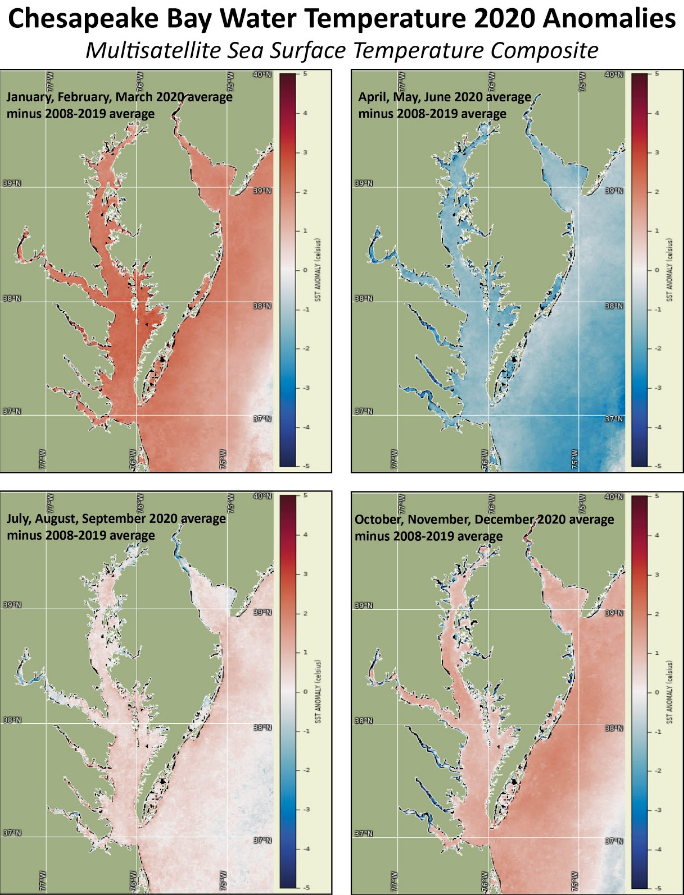
\includegraphics[width=0.49\linewidth]{images/ches-temp-temp} \includegraphics[width=0.49\linewidth]{SOE-MAFMC-2021_files/figure-latex/ches-temp-2} \caption{Left panel: Chesapeake Bay sea surface temperature (SST) seasonal spatial anomalies for 2020, from NOAA multisatellite SST composite. Positive values (red) above 2008-2019 average; negative values (blue) below 2008-2019 average. A) Jan, Feb, Mar; B) Apr, May, Jun; C) Jul, Aug, Sep; D) Oct, Nov, Dec. Right panel: NOAA Chesapeake Bay Interpretive Buoy System Gooses Reef bouy sea water temperature; Blue = 2020, red = Long term average 2010-2019.}\label{fig:ches-temp}
\end{figure}

A marine heatwave is a warming event that lasts for five or more days
with sea surface temperatures above the 90th percentile of the
historical daily climatology (1982-2011)
{[}\protect\hyperlink{ref-hobday_hierarchical_2016}{11}{]}. The MAB
experienced frequent ocean heatwaves of moderate intensity in 2020 that
extended well into December (Fig. \ref{fig:heatwave-year}), similar to
warming observed in Chesapeake Bay (Fig. \ref{fig:ches-temp}).

\begin{figure}

{\centering \includegraphics{SOE-MAFMC-2021_files/figure-latex/heatwave-year-1} 

}

\caption{Marine heatwave events (red) in the Mid-Atlantic occuring in 2020.}\label{fig:heatwave-year}
\end{figure}

Changes in ocean temperature and circulation alter habitat features such
as the cold pool, a 20--60 m thick band of cold, relatively uniform
near‐bottom water that persists from spring to fall over the mid-shelf
and outer shelf of the Middle Atlantic Bight (MAB) and Southern Flank of
Georges Bank {[}\protect\hyperlink{ref-lentz_seasonal_2017}{12}{]}. The
cold pool plays an essential role in the structuring of the MAB
ecosystem. It is a reservoir of nutrients that feeds phytoplankton
productivity, is essential fish spawning and nursery habitat, and
affects fish distribution and behavior
{[}\protect\hyperlink{ref-lentz_seasonal_2017}{12}{]}. The average
temperature of the cold pool has been getting warmer over time
{[}\protect\hyperlink{ref-miller_state-space_2016}{13}{]}). These
changes can affect distribution and migration timing for species that
depend on the cold pool habitat. The area of the MAB cold pool was near
average in 2018 (Fig. \ref{fig:cold-pool-map}), the last complete year
of the dataset. The size of the cold pool varies annually, with the
smallest sizes associated with record-warm years (e.g.~2012). The cold
pool temperature shows a similar variation as its extent, both of which
are strongly impacted by each early spring setting in temperature on the
shelf.

\begin{figure}

{\centering 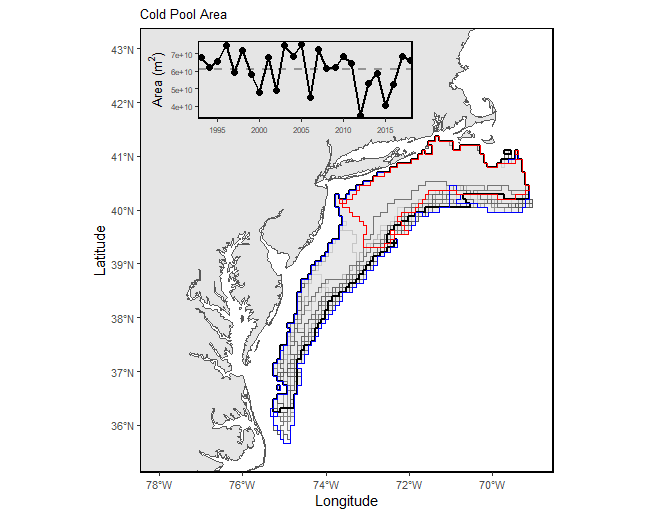
\includegraphics[width=8.97in]{images/cold_pool_area} 

}

\caption{Map of cold pool area. Time series of cold pool spatial extent from1993-2018. Black = 2018 (Last year in time series), Red = 2012 Minimum area, Blue = 2005 Maximum area.}\label{fig:cold-pool-map}
\end{figure}

New glider-based observations revealed areas of low pH (7.8) during
summer in Mid-Atlantic habitats occupied by Atlantic surfclams and sea
scallops (Fig. \ref{fig:mab-oa})
{[}\protect\hyperlink{ref-wrightfairbanks_autonomous_2020}{14}{]}. This
seasonal pH minimum is associated with cold-pool subsurface and bottom
water, which is cut off from mixing with surface water by strong
stratification. However, seawater pH in shelf waters increased during
the fall mixing period due to the influence of a slope water mass
characterized by warm, salty, highly alkaline seawater. Lower pH in
nearshore waters is likely associated with freshwater input.

\begin{figure}

{\centering 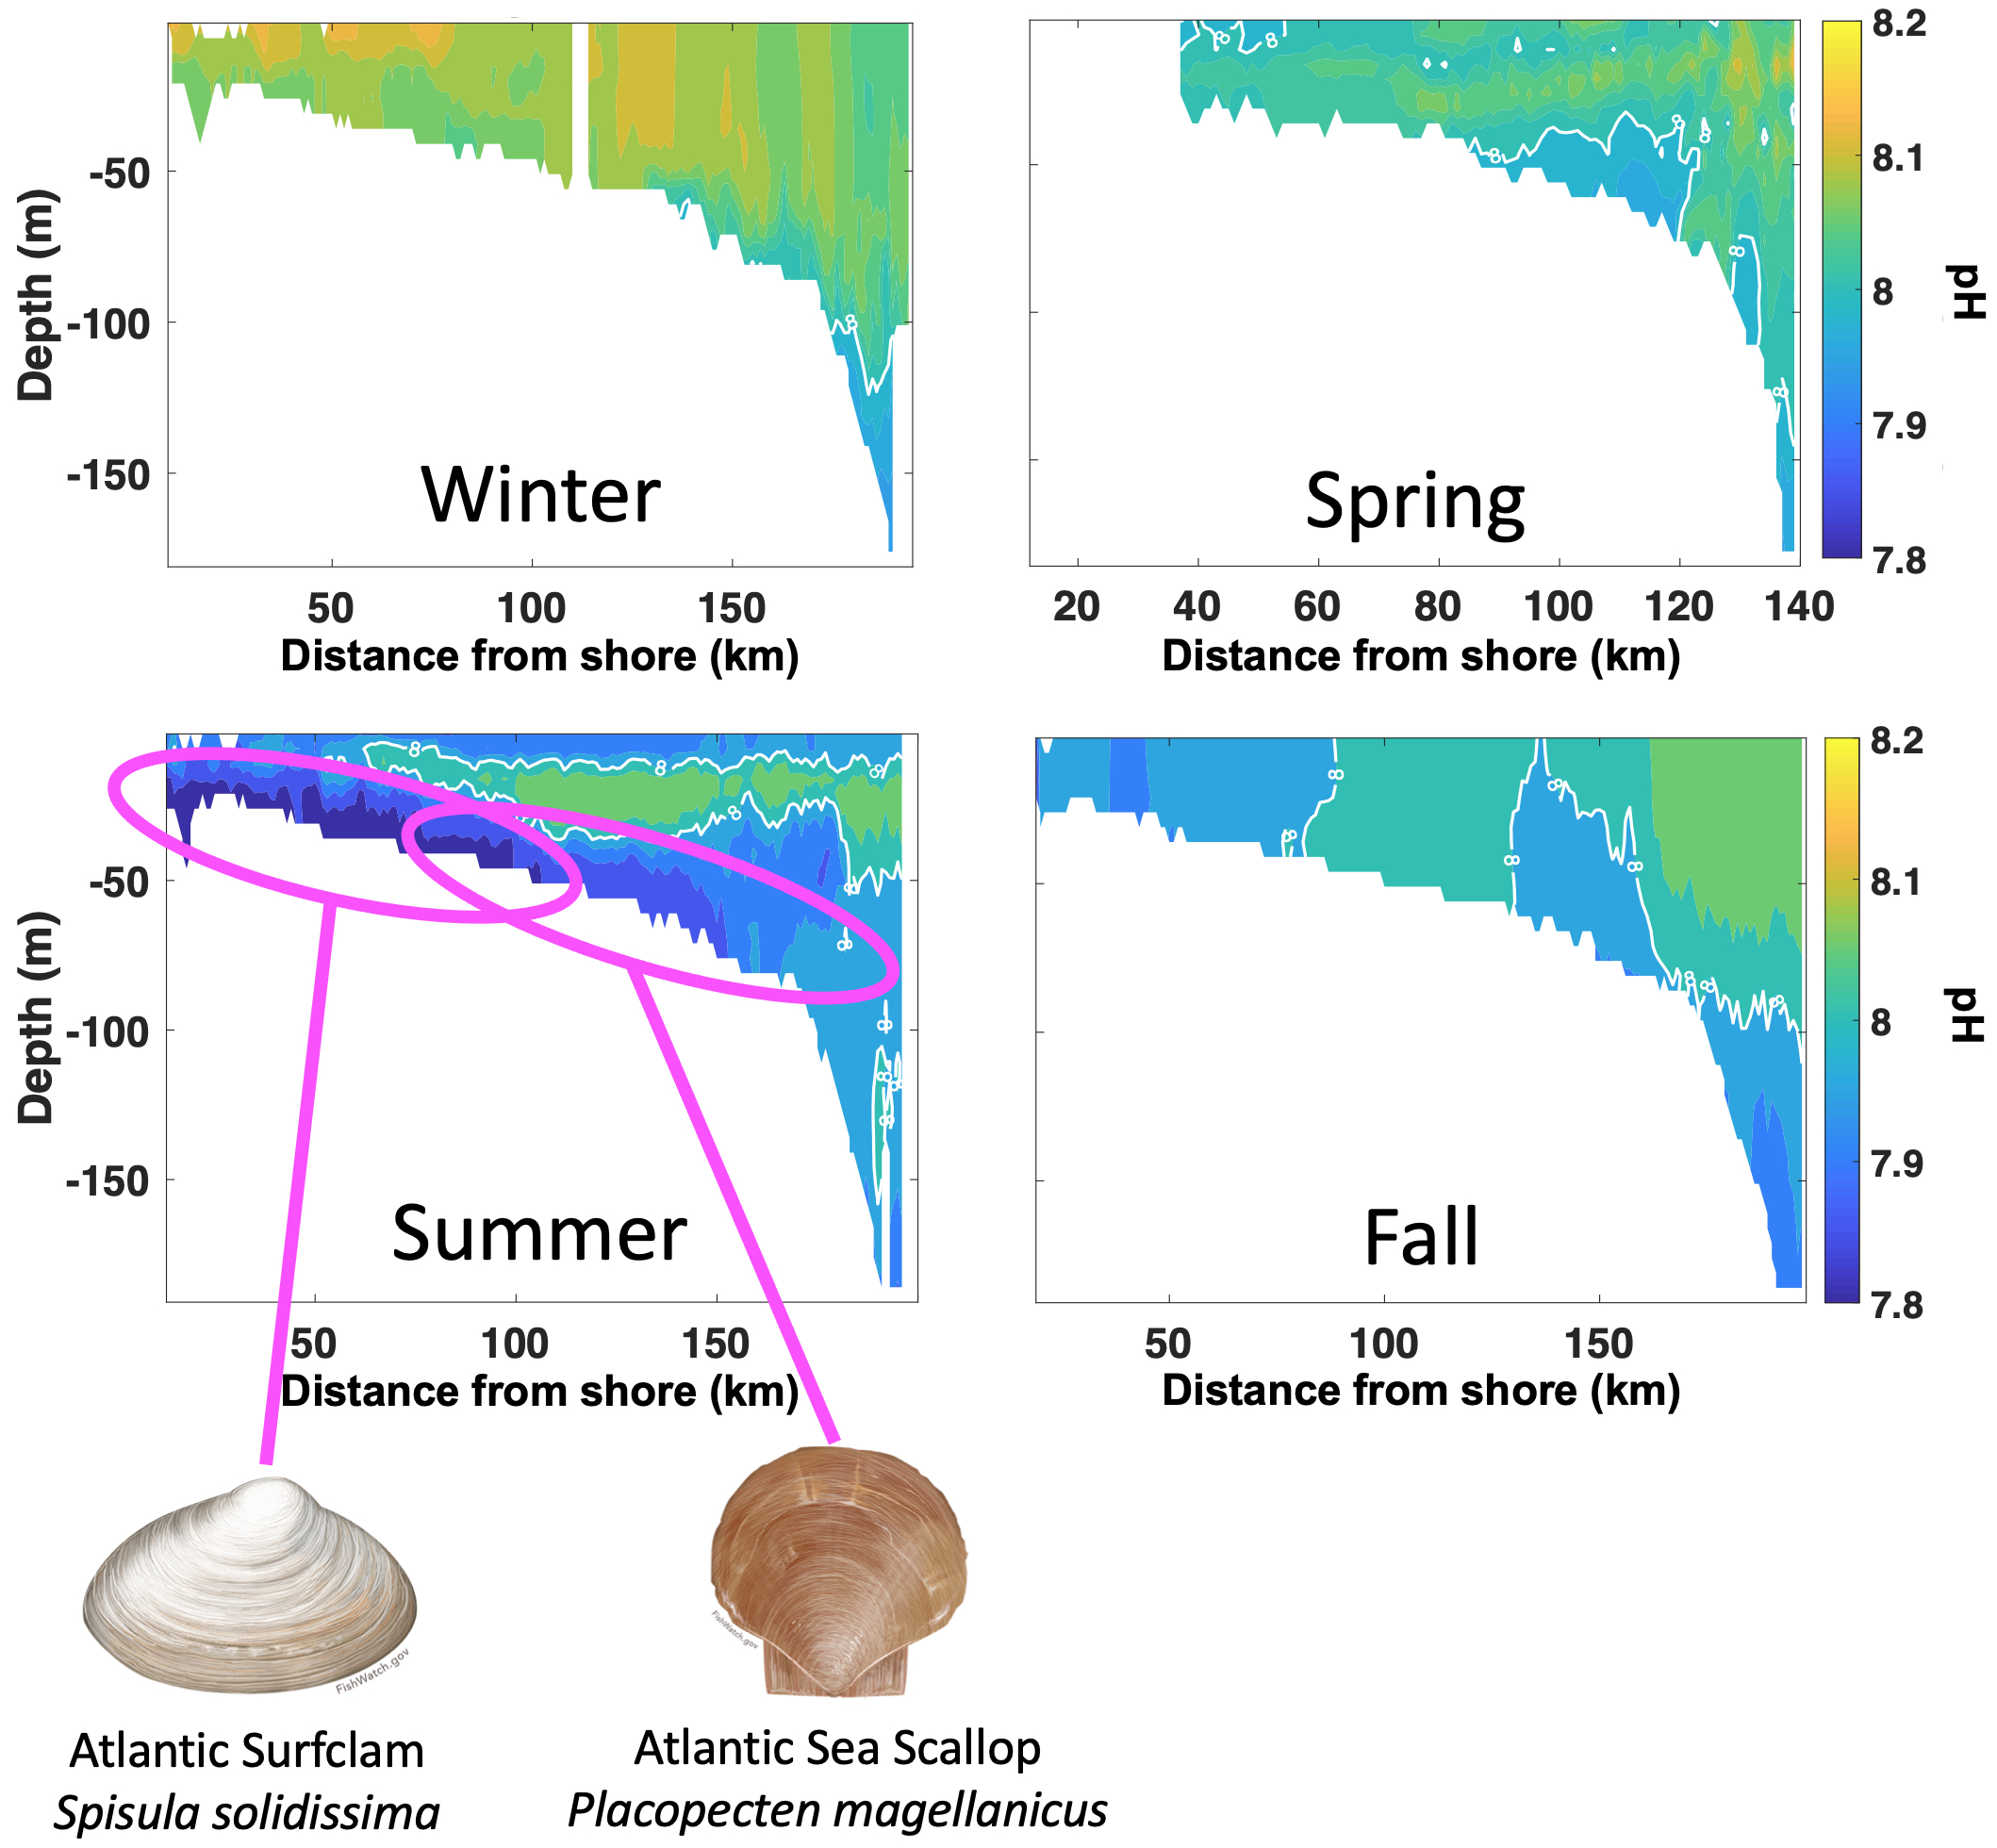
\includegraphics[width=0.7\linewidth]{images/Seasonal pH on MAB shelf - Grace Saba} 

}

\caption{ Seasonal glider-based pH observations on the Mid-Atlantic Bight shelf (New Jersey cross-shelf transect) in relation to Atlantic surfclam and Atlantic sea scallop habitats (modified from Wright-Fairbanks et al. 2020).}\label{fig:mab-oa}
\end{figure}

\hypertarget{ecosystem-productivity-indicators-primary-production-zooplankton-forage-fish-fish-condition}{%
\subsubsection{Ecosystem Productivity Indicators: primary production,
zooplankton, forage fish, fish
condition}\label{ecosystem-productivity-indicators-primary-production-zooplankton-forage-fish-fish-condition}}

Increased temperatures, as reported above, can increase the rate of
photosynthesis by phytoplankton (i.e.~primary productivity). Annual
primary production has increased over time, primarily driven by
increased productivity in the summer months (Figs. \ref{fig:pp-monthly},
\ref{fig:chl-weekly}).

\begin{figure}

{\centering \includegraphics{SOE-MAFMC-2021_files/figure-latex/pp-monthly-1} 

}

\caption{Monthly primary production trends show the annual cycle (i.e. the peak during the summer months) and the changes over time for each month.}\label{fig:pp-monthly}
\end{figure}

Larger-than-average phytoplankton blooms were observed from late fall
into winter in 2020 (Fig. \ref{fig:chl-weekly}).

\begin{figure}

{\centering \includegraphics{SOE-MAFMC-2021_files/figure-latex/chl-weekly-1} 

}

\caption{Weekly chlorophyll concentrations and primary productivity in the Mid-Atlantic are shown for by the colored line for 2020 (dashed portion indicates preliminary data from a new satellite source). The long-term mean is shown in black and shading indicates +/- 1 sample SD.}\label{fig:chl-weekly}
\end{figure}

Climatology of seasonal phytoplankton size fractions confirms that the
phytoplankton community in the summer is dominated by smaller (pico and
nano) size classes (Fig. \ref{fig:weekly-phyto-size}). This implies less
efficient transfer of primary production to higher trophic levels.

\begin{figure}

{\centering \includegraphics{SOE-MAFMC-2021_files/figure-latex/weekly-phyto-size-1} 

}

\caption{The annual climatology (1998-2019) percent composition of the phytoplankton size classes in the Mid-Atlantic bight based on satellite observations.}\label{fig:weekly-phyto-size}
\end{figure}

Trends in gelatinous zooplankton and krill are the same across
ecological production units (EPUs) as last year (data were updated to
2019; Fig. \ref{fig:zoo-strat-abun}). There has been a long term
increase in both groups on Georges Bank and for krill in the Gulf of
Maine as well.

\begin{figure}

{\centering \includegraphics{SOE-MAFMC-2021_files/figure-latex/zoo-strat-abun-1} 

}

\caption{Stratified abundance of cnidarians and euphausiids in Mid-Atlantic Bight.}\label{fig:zoo-strat-abun}
\end{figure}

Larger zooplankton (i.e.~\emph{Calanus finmarchicus}) had above average
abundance in 2018-2019, while smaller-bodied copepods were near or below
average (Fig. \ref{fig:zoo-abund}).

\begin{figure}

{\centering \includegraphics{SOE-MAFMC-2021_files/figure-latex/zoo-abund-1} 

}

\caption{Large (red) and small-bodied (blue) copepod abundance in the Mid-Atlantic Bight.}\label{fig:zoo-abund}
\end{figure}

An index of aggregate zooplankton and forage fish fluctuations (forage
anomaly) constructed from zooplankton and ichthyoplankton data has no
apparent trend in MAB, but appears to be more variable since 2010 (Fig.
\ref{fig:forage-anomaly}). Changes in environmental conditions, lower
tropic levels, and diversity of the plankton community are potentially
impacting the prey of zooplankton and ichthyoplankton, which may affect
this index.

\begin{figure}

{\centering \includegraphics{SOE-MAFMC-2021_files/figure-latex/forage-anomaly-1} 

}

\caption{Changes from 2000-2019 average abundance for an aggregate of 13 zooplankton and 16 ichthyoplankton groups sampled on NEFSC ECOMON surveys.}\label{fig:forage-anomaly}
\end{figure}

Nutritional value (energy content) of juvenile and adult forage fishes
as prey is related to both environmental conditions, fish growth and
reproductive cycles. Forage energy density measurements from NEFSC trawl
surveys 2017-2019 are building toward a time series to evaluate trends
(Fig. \ref{fig:energy-density}). New 2019 measurements were consistent
with last year's report: the energy density of Atlantic herring was
almost half the value (5.69 +/- 0.07 kJ/g wet weight) reported in
earlier studies (10.6-9.4 kJ/ g wet weight). Silver hake, sandlance,
longfin squid (\emph{Loligo} below) and shortfin squid (\emph{Illex}
below) were also lower than previous estimates
{[}\protect\hyperlink{ref-steimle_energy_1985}{15},\protect\hyperlink{ref-lawson_important_1998}{16}{]}.
Energy density of alewife, butterfish and Atlantic mackerel varies
seasonally, with seasonal estimates both higher and lower than estimates
from previous decades.

\begin{figure}

{\centering \includegraphics{SOE-MAFMC-2021_files/figure-latex/energy-density-1} 

}

\caption{Forage fish mean energy density mean and standard deviation by season and year, compared with 1980s (Steimle and Terranove 1985) and 1990s (Lawson et al. 1998) values.}\label{fig:energy-density}
\end{figure}

The health and well being of individual fish can be related to body
shape condition indices (i.e.~weight at a given length) such as relative
condition index, which is the ratio of observed weight to predicted
weight based on length
{[}\protect\hyperlink{ref-le_cren_length-weight_1951}{17}{]}. Heavier
and fatter fish at a given length have higher relative condition which
is expected to influence growth, reproductive output and survival. A
pattern of generally good condition was observed across many MAB species
prior to 2000, followed by a period of generally poor condition from
2001-2010, with a mix of good and poor condition 2011-2019 (Fig.
\ref{fig:mab-cf}). While there were no new data to update the condition
indicator this year, preliminary results of synthetic analyses described
in the
\protect\hyperlink{environmental-drivers-of-fish-condition}{Implications
section} show that changes in fishing pressure, population size,
temperature, and zooplankton influence the condition of different fish
species. Potential links between fish condition, fisheries, and markets
are under investigation.

\begin{figure}

{\centering 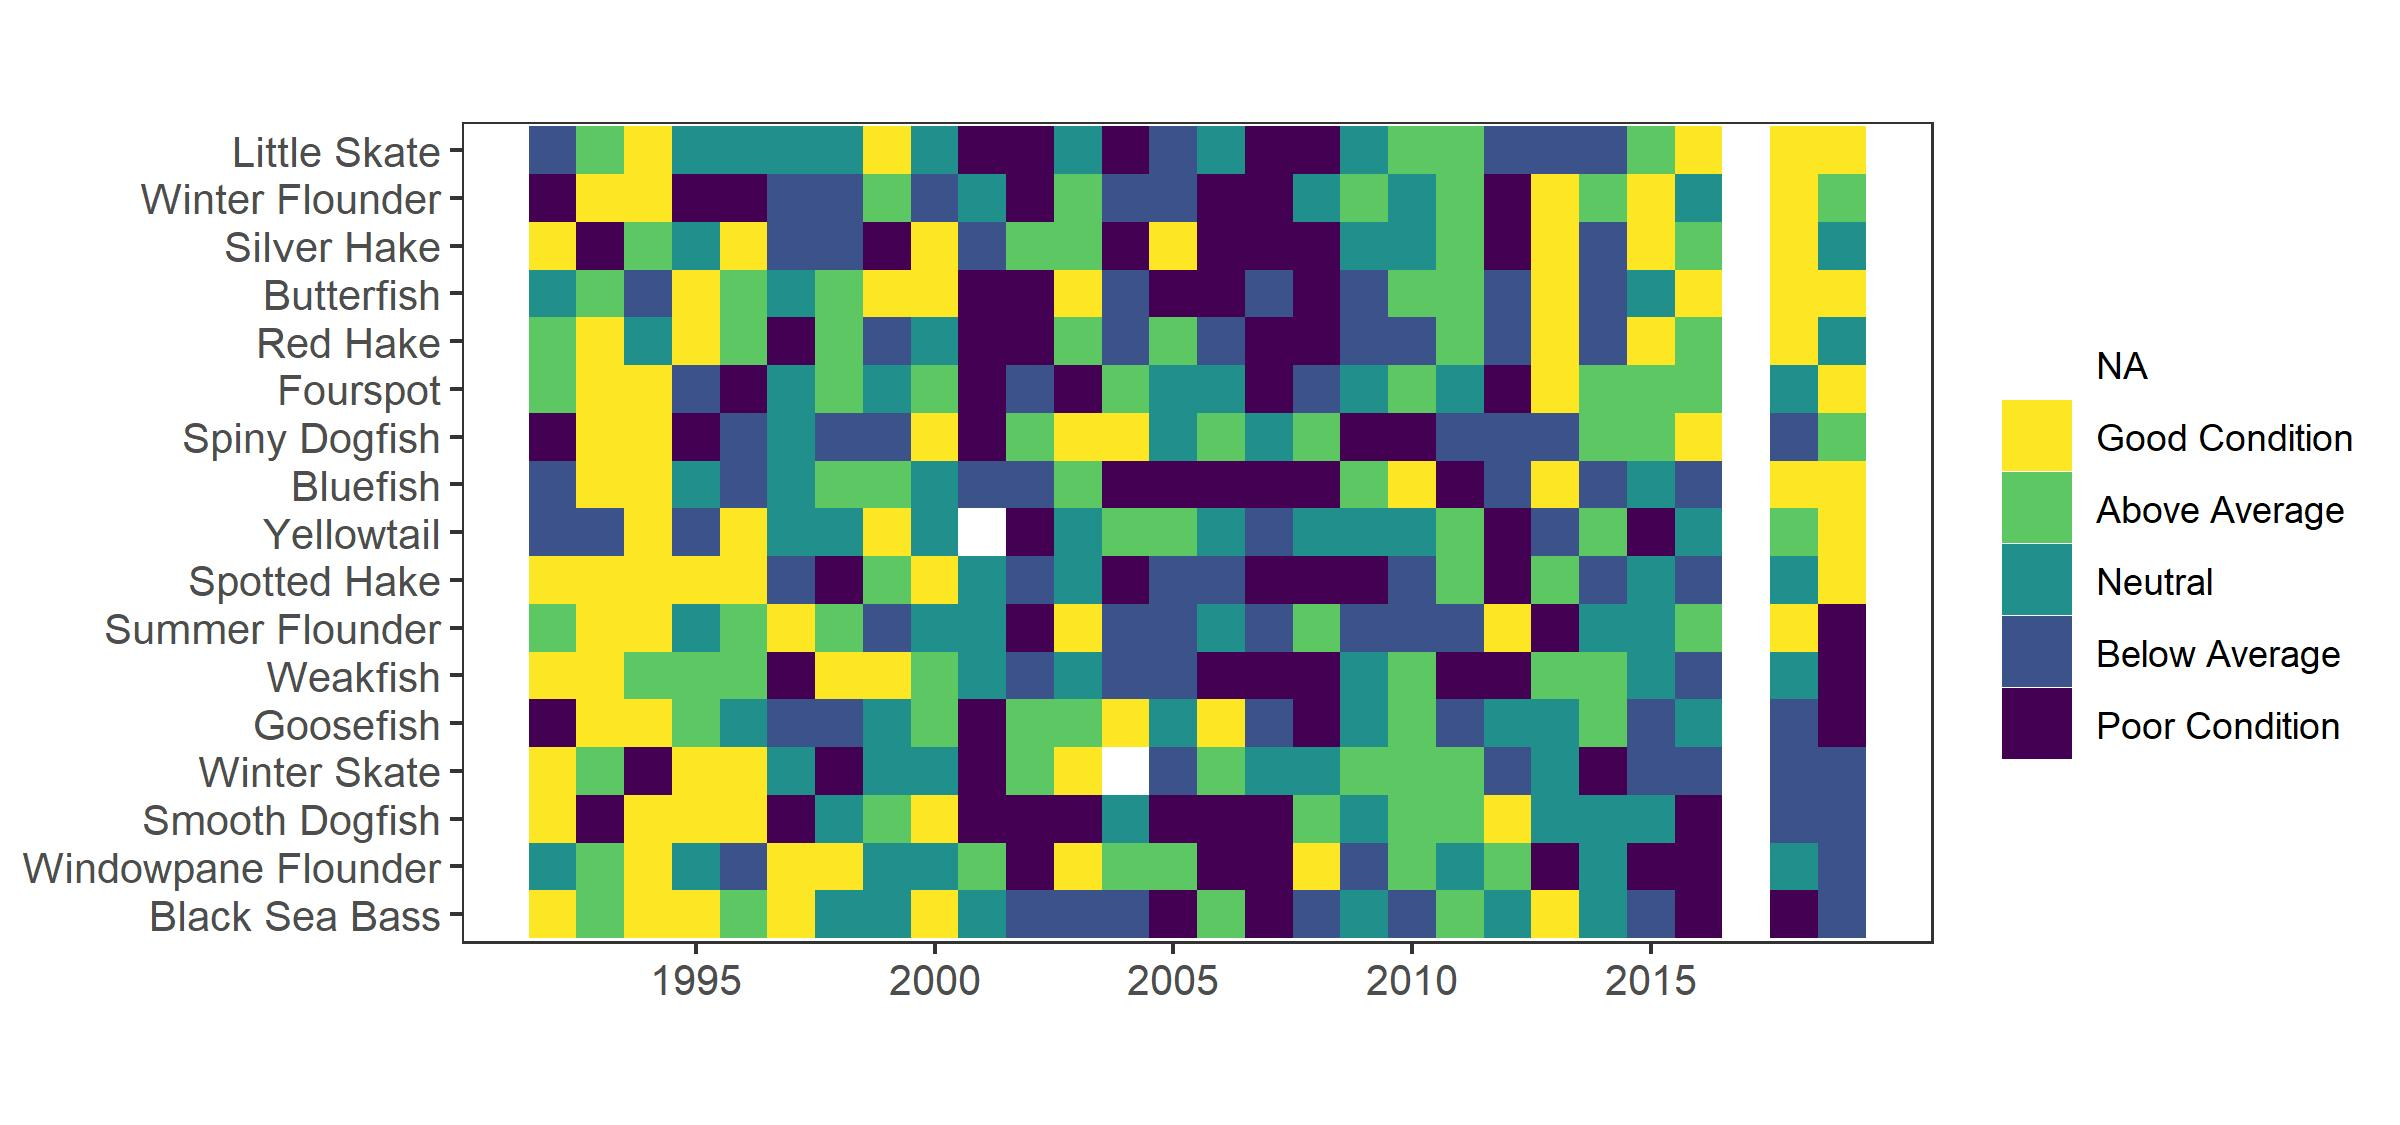
\includegraphics[width=1\linewidth]{images/MABcondition_2019_viridis_final} 

}

\caption{Condition factor for fish species in the MAB based on fall NEFSC bottom trawl survey data. MAB data are missing for 2017 due to survey delays, and no survey was conducted in 2020.}\label{fig:mab-cf}
\end{figure}

\hypertarget{ecosystem-structure-indicators-distribution-shifts-diversity-predators}{%
\subsubsection{Ecosystem Structure Indicators: distribution shifts,
diversity,
predators}\label{ecosystem-structure-indicators-distribution-shifts-diversity-predators}}

As noted in the \protect\hyperlink{implications}{Landings Implications
section above}, stocks are shifting distribution throughout the region.
In aggregate, fish stocks are moving northeast along the shelf and into
deeper waters.

Zooplankton diversity is increasing in the MAB, while larval fish and
adult fish diversity indices are stable over time with current values
near the long-term average (see
\protect\hyperlink{ecological-diversity}{Diversity Indicators section,
above}).

New indicators for shark populations, combined with information on gray
seals (see \protect\hyperlink{protected-species}{Protected Species
Implications section, above}), suggests predator populations range from
stable (sharks, Figs. \ref{fig:observed-sharks},
\ref{fig:hms-cpue-sharks}) to increasing (seals) in the MAB. Stable
predator populations suggest stable predation pressure on managed
species, but increasing predator populations may reflect increasing
predation pressure.

\begin{figure}

{\centering \includegraphics{SOE-MAFMC-2021_files/figure-latex/observed-sharks-1} 

}

\caption{Estimated number of sharks per unit effort from Northeast Fisheries Observer Program data.}\label{fig:observed-sharks}
\end{figure}

\begin{figure}

{\centering \includegraphics{SOE-MAFMC-2021_files/figure-latex/hms-cpue-sharks-1} 

}

\caption{Estimated number of sharks per unit effort from Highly Migratory Species Pelagic Observer Program data.}\label{fig:hms-cpue-sharks}
\end{figure}

As noted in the \protect\hyperlink{protected-species}{Protected Species
section}, gray seal populations are increasing. Harbor and gray seals
occupying New England waters are generalist predators that consume more
than 30 different prey species. An evaluation of hard parts found in
seal stomachs showed that harbor and gray seals predominantly exploit
abundant demersal fish species (i.e.~red, white and silver hake). Other
relatively abundant prey species found in hard-part remains include sand
lance, yellowtail flounder, four-spotted flounder, Gulf-stream flounder,
haddock, herring, redfish, and squids.

A recent stable isotope study utilizing gray seal scat samples obtained
from Massachusetts habitats showed individual gray seals can specialize
on particular prey. It also found that gray seals vary their diet
seasonally, focusing on demersal inshore species prior to the spring
molt, and offshore species such as sand lance after molting. DNA studies
on gray seal diet in Gulf of Maine and Massachusetts waters found spiny
dogfish and Jonah crab present in gray seal scat samples. Skate and crab
remains were also found in gray seal stomach remains. In contrast to
direct feeding, it is uncertain if the presence of skates and crabs is
due to secondary consumption or scavenging.

\hypertarget{habitat-climate-vulnerability}{%
\subsubsection{Habitat Climate
Vulnerability}\label{habitat-climate-vulnerability}}

A recent habitat climate vulnerability analysis links black sea bass,
scup, and summer flounder to several highly vulnerable nearshore
habitats from salt marsh through shallow estuarine and marine reefs.
Details on highly vulnerable habitats with linkages to a variety of
species, including which life stages have different levels of dependence
on a particular habitat, are available in a detailed table.\footnote{\url{https://noaa-edab.github.io/ecodata/Hab_table}}

\hypertarget{implications-6}{%
\subsubsection{Implications}\label{implications-6}}

\hypertarget{links-between-climate-change-and-managed-species}{%
\paragraph{Links between climate change and managed
species}\label{links-between-climate-change-and-managed-species}}

Estuarine and nearshore habitats support many life stages of state and
federally-managed species, and are highly vulnerable to climate change.
Below we highlight how recently observed habitat changes affect several
key managed species in Chesapeake Bay and in both nearshore and offshore
waters of the MAB. Overall, multiple drivers interact differently for
each species, producing a range of population impacts.

\hypertarget{striped-bass-and-blue-crabs}{%
\subparagraph{\texorpdfstring{\emph{Striped bass and blue
crabs}}{Striped bass and blue crabs}}\label{striped-bass-and-blue-crabs}}

The warmer than average winter may have affected key Chesapeake Bay
fishery resources during a critical period. Results of the Maryland
juvenile striped bass survey, conducted by the Maryland Department of
Natural Resources (MDNR), showed low recruitment success in
\href{https://news.maryland.gov/dnr/2020/10/13/chesapeake-bay-young-of-year-survey-results-released/}{2020},
about fivefold below the long-term average. This low recruitment event
may have been caused by a mismatch in striped bass larval and prey
abundance due to the warm winter conditions, resulting in reduced larval
survival. Warm winters typically trigger early phytoplankton and
zooplankton blooms, including key copepod prey, which die before striped
bass larvae are present in the tributary
{[}\protect\hyperlink{ref-millette_water_2020}{18}{]}.

In addition to winter water temperature, survival of early life stages
of striped bass in the Chesapeake Bay is strongly correlated with
freshwater flow
{[}\protect\hyperlink{ref-millette_water_2020}{18}--\protect\hyperlink{ref-north_linking_2003}{20}{]}.
High-flow regimes push zooplankton prey downstream, where they get
trapped with striped bass larvae in the estuarine turbidity maximum. In
low-flow years, such as 2020, zooplankton prey are less likely to match
up with striped bass larvae in space and time, reducing striped bass
larval survival and recruitment success. The combined effects of warm
winter temperatures and low flow in 2020 may be the primary cause of the
low recruitment observed by the MDNR juvenile striped bass survey.

Conversely, warmer winter temperatures may have reduced overwintering
mortality of Chesapeake Bay blue crabs. Calculations done by MDNR based
on data from the annual bay-wide winter dredge survey indicate that blue
crabs experienced the lowest overwintering mortality ever observed
(\href{https://www.chesapeakebay.net/documents/2020_Blue_Crab_Advisory_Report_Final_06-22-20.pdf}{2020
Chesapeake Bay Blue Crab Advisory Report}). Previous studies have
demonstrated the correlation between winter water temperature and blue
crab survival in the Chesapeake Bay
{[}\protect\hyperlink{ref-bauer_temperature-_2010}{21}--\protect\hyperlink{ref-rome_linking_2005}{23}{]}.

\hypertarget{american-oyster}{%
\subparagraph{\texorpdfstring{\emph{American
oyster}}{American oyster}}\label{american-oyster}}

Increased salinity in the Chesapeake Bay often results in high juvenile
oyster abundance
{[}\protect\hyperlink{ref-kimmel_relationship_2014}{24}{]}. In Maryland,
the 2020 MDNR fall oyster survey documented above-average spatsets along
the Eastern Shore as expected, given the high salinity. However, the
Western Shore did not fare as well, suggesting that local environmental
conditions are also important.

\hypertarget{summer-flounder}{%
\subparagraph{\texorpdfstring{\emph{Summer
flounder}}{Summer flounder}}\label{summer-flounder}}

The NEAMAP survey saw a doubling of summer flounder catch in the near
coastal waters in 2020 relative to 2019. It is more likely that
environmental conditions made summer flounder more available in
nearshore habitats and less likely that the population doubled between
2019 and 2020, but this remains to be confirmed and investigated along
with habitat-specific information. In upcoming reports, we plan to
integrate information on federally managed species in both Chesapeaky
Bay (ChesMMAP) and NEAMAP surveys with nearshore environmental
information to highlight interactions in these important habitats.

\hypertarget{surfclam}{%
\subparagraph{\texorpdfstring{\emph{Surfclam}}{Surfclam}}\label{surfclam}}

Ocean acidification also has different implications, depending on the
species and life stage. Recent lab studies have found that surfclams
exhibited metabolic depression in a pH range of 7.46-7.28
{[}\protect\hyperlink{ref-pousse_energetic_2020}{25}{]}. In other
bivalve species, metabolic depression happened between pH 7.38 and 7.14
for blue mussels {[}\protect\hyperlink{ref-thomsen_moderate_2010}{26}{]}
and around pH 7.1 for Pacific oysters
{[}\protect\hyperlink{ref-lannig_impact_2010}{27}{]}. At pH of 7.51,
short term experiments indicated that surfclams were selecting particles
differently, which may have long term implications for growth
{[}\protect\hyperlink{ref-pousse_energetic_2020}{25}{]}. Computer models
would help in determining the long term implications of growth on
surfclam populations. Data from about one year of observations
(2018-2019) show that seasonal ocean pH has not yet reached the
metabolic depression threshold observed for surfclams in lab studies so
far; however, thresholds at different life stages, specifically larval
stages that are typically more vulnerable to ocean acidification, have
not yet been determined.

\hypertarget{heatwave-impacts}{%
\paragraph{Heatwave impacts}\label{heatwave-impacts}}

Marine heatwaves measure not just temperature, but how long the
ecosystem is subjected to the high temperature. They are driven by both
atmospheric and oceanographic factors and can have dramatic impacts on
marine ecosystems. Marine heatwaves are measured in terms of intensity
(water temperature) and duration (the cumulative number of degree days)
using satellite measurements of daily sea surface temperature. Plotted
below are maximum intensity and cumulative intensity, which is intensity
times duration.

The MAB had multiple marine heatwaves in 2020 (Fig.
\ref{fig:heatwave-year}). Although the individual maximum intensity
heatwave on July 28 was near intensity average (for a heatwave), the
combination of multiple heatwaves led to the third highest cumulative
heatwave intensity on record in 2020 (Fig. \ref{fig:heatwave}). The
strongest heatwaves on record in the Middle Atlantic Bight occurred in
the winter of 2012 in terms of maximum intensity (+5.13 °C above
average) and in the winter/summer of 2012 in terms of cumulative
intensity (515 °C-days). 2012 is still the warmest year on record in the
Northeast US LME. Recent papers published on the impacts of the 2012
heatwave give insight into the implications of marine heatwaves. Lobster
was impacted as well as the timing of fishing and markets
{[}\protect\hyperlink{ref-mills_fisheries_2013}{28}{]}. Other more
southern warm water species have been observed in the MAB, including
reports in 2020 of Cobia in the waters off of Rhode Island.

\begin{figure}

{\centering \includegraphics{SOE-MAFMC-2021_files/figure-latex/heatwave-1} 

}

\caption{Marine heatwave cumulative intesity (left) and maximum intensity (right) in the Mid-Atlantic Bight.}\label{fig:heatwave}
\end{figure}

\hypertarget{distribution-shift-impacts}{%
\paragraph{Distribution shift
impacts}\label{distribution-shift-impacts}}

Trends for a suite of 48 commercially or ecologically important fish
species along the entire Northeast Shelf continue to show movement
towards the northeast and generally into deeper water (Fig.
\ref{fig:species-dist}). We hope to expand this analysis beyond fish.
Marine mammal distribution maps are available online\footnote{\url{https://www.nefsc.noaa.gov/AMAPPSviewer/}};
updated maps and trends are currently being developed.

Shifting species distributions alter both species interactions and
fishery interactions. In particular, shifting species distributions can
alter expected management outcomes from spatial allocations and bycatch
measures based on historical fish and protected species distributions.

\hypertarget{ecosystem-productivity-change-impacts}{%
\paragraph{Ecosystem productivity change
impacts}\label{ecosystem-productivity-change-impacts}}

Climate and associated changes in the physical environment affect
ecosystem productivity, with warming waters increasing the rate of
photosynthesis at the base of the food web. However, increased summer
production in the MAB may not translate to increased fish biomass
because smaller phytoplankton dominate in this season.

While krill and large gelatinous zooplankton are increasing over time,
smaller zooplankton are periodically shifting abundance between the
larger, more nutritious Calanus finmarchicus and smaller bodied copepods
with no apparent overall trend. Forage species are difficult to survey,
but a new index that includes ichthyoplankton suggests high interannual
variability in abundance of larval fish and zooplankton prey. The
nutritional content of larger bodied forage fish and squid changes
seasonally in response to ecosystem conditions, with apparent declines
in energy density for Atlantic herring and \emph{Illex} squid relative
to the 1980s, but similar energy density for other forage species. Some
of these factors are now being linked to the relative condition of
managed fish.

\hypertarget{environmental-drivers-of-fish-condition}{%
\subparagraph{\texorpdfstring{\emph{Environmental drivers of fish
condition}}{Environmental drivers of fish condition}}\label{environmental-drivers-of-fish-condition}}

Generalized Additive Models (GAMs) were used to test how measures of
fishing pressure, stock abundance, and individual environmental
variables performed in explaining the changes of fish condition
(fatness) over time. Some species such as Acadian redfish, butterfish
and winter flounder were more affected by fishing pressure and stock
size, whereas other species such as weakfish, windowpane flounder, and
American plaice may be more affected by local bottom temperatures and
zooplankton.

These relationships can potentially provide insights on which species
may be more vulnerable to environmental changes such as climate change,
as well as what biomass changes may be expected from certain species
given current environmental conditions.

Correlations were examined between environmental drivers, and as
expected there were strong temperature correlations between seasons as
well as correlations between temperature and zooplankton indices.
Planned future work includes building full GAM models for each fish
species, and linking fish condition to socio-economic models to assess
whether fish condition impacts the market value generated by that
species.

\hypertarget{potential-economic-impacts-of-fish-condition}{%
\subparagraph{\texorpdfstring{\emph{Potential economic impacts of fish
condition}}{Potential economic impacts of fish condition}}\label{potential-economic-impacts-of-fish-condition}}

Economic theory and empirical analyses have highlighted that many
factors can affect the price of fish, including the total quantity of
fish in the market (sometimes including internationally), increased
demand around holidays, time the fish was in storage, and other issues
that either affect the quality of the fish or the amount of fish
available for purchase. We plan on empirically exploring whether fish
condition is a quality metric that drives fish prices. Understanding the
socio-economic impact of fish condition will help us more holistically
understand the impacts of condition change on society, if any.

\hypertarget{other-ocean-uses-offshore-wind}{%
\subsection{Other Ocean Uses: Offshore
Wind}\label{other-ocean-uses-offshore-wind}}

\hypertarget{indicators-development-timeline-revenue-in-lease-areas-survey-overlap}{%
\subsubsection{Indicators: development timeline, revenue in lease areas,
survey
overlap}\label{indicators-development-timeline-revenue-in-lease-areas-survey-overlap}}

More than 20 offshore wind development projects are proposed for
construction over the next decade in the Northeast (projects \&
construction timelines based on Table E-4 of South Fork Wind Farm Draft
Environmental Impact Statement). Offshore wind areas may cover more than
1.7 million acres by 2030 (Fig. \ref{fig:wind-dev-cumul}). Just over
1,900 foundations and more than 3,000 miles of inter-array and offshore
export cables are proposed to date. Each proposed project has a two-year
construction timeline
{[}\protect\hyperlink{ref-boem_bureau_2021}{29}{]}. Based on current
timelines, the areas affected would be spread out such that it is
unlikely that any one particular area would experience full development
at one time.\\

\begin{figure}

{\centering 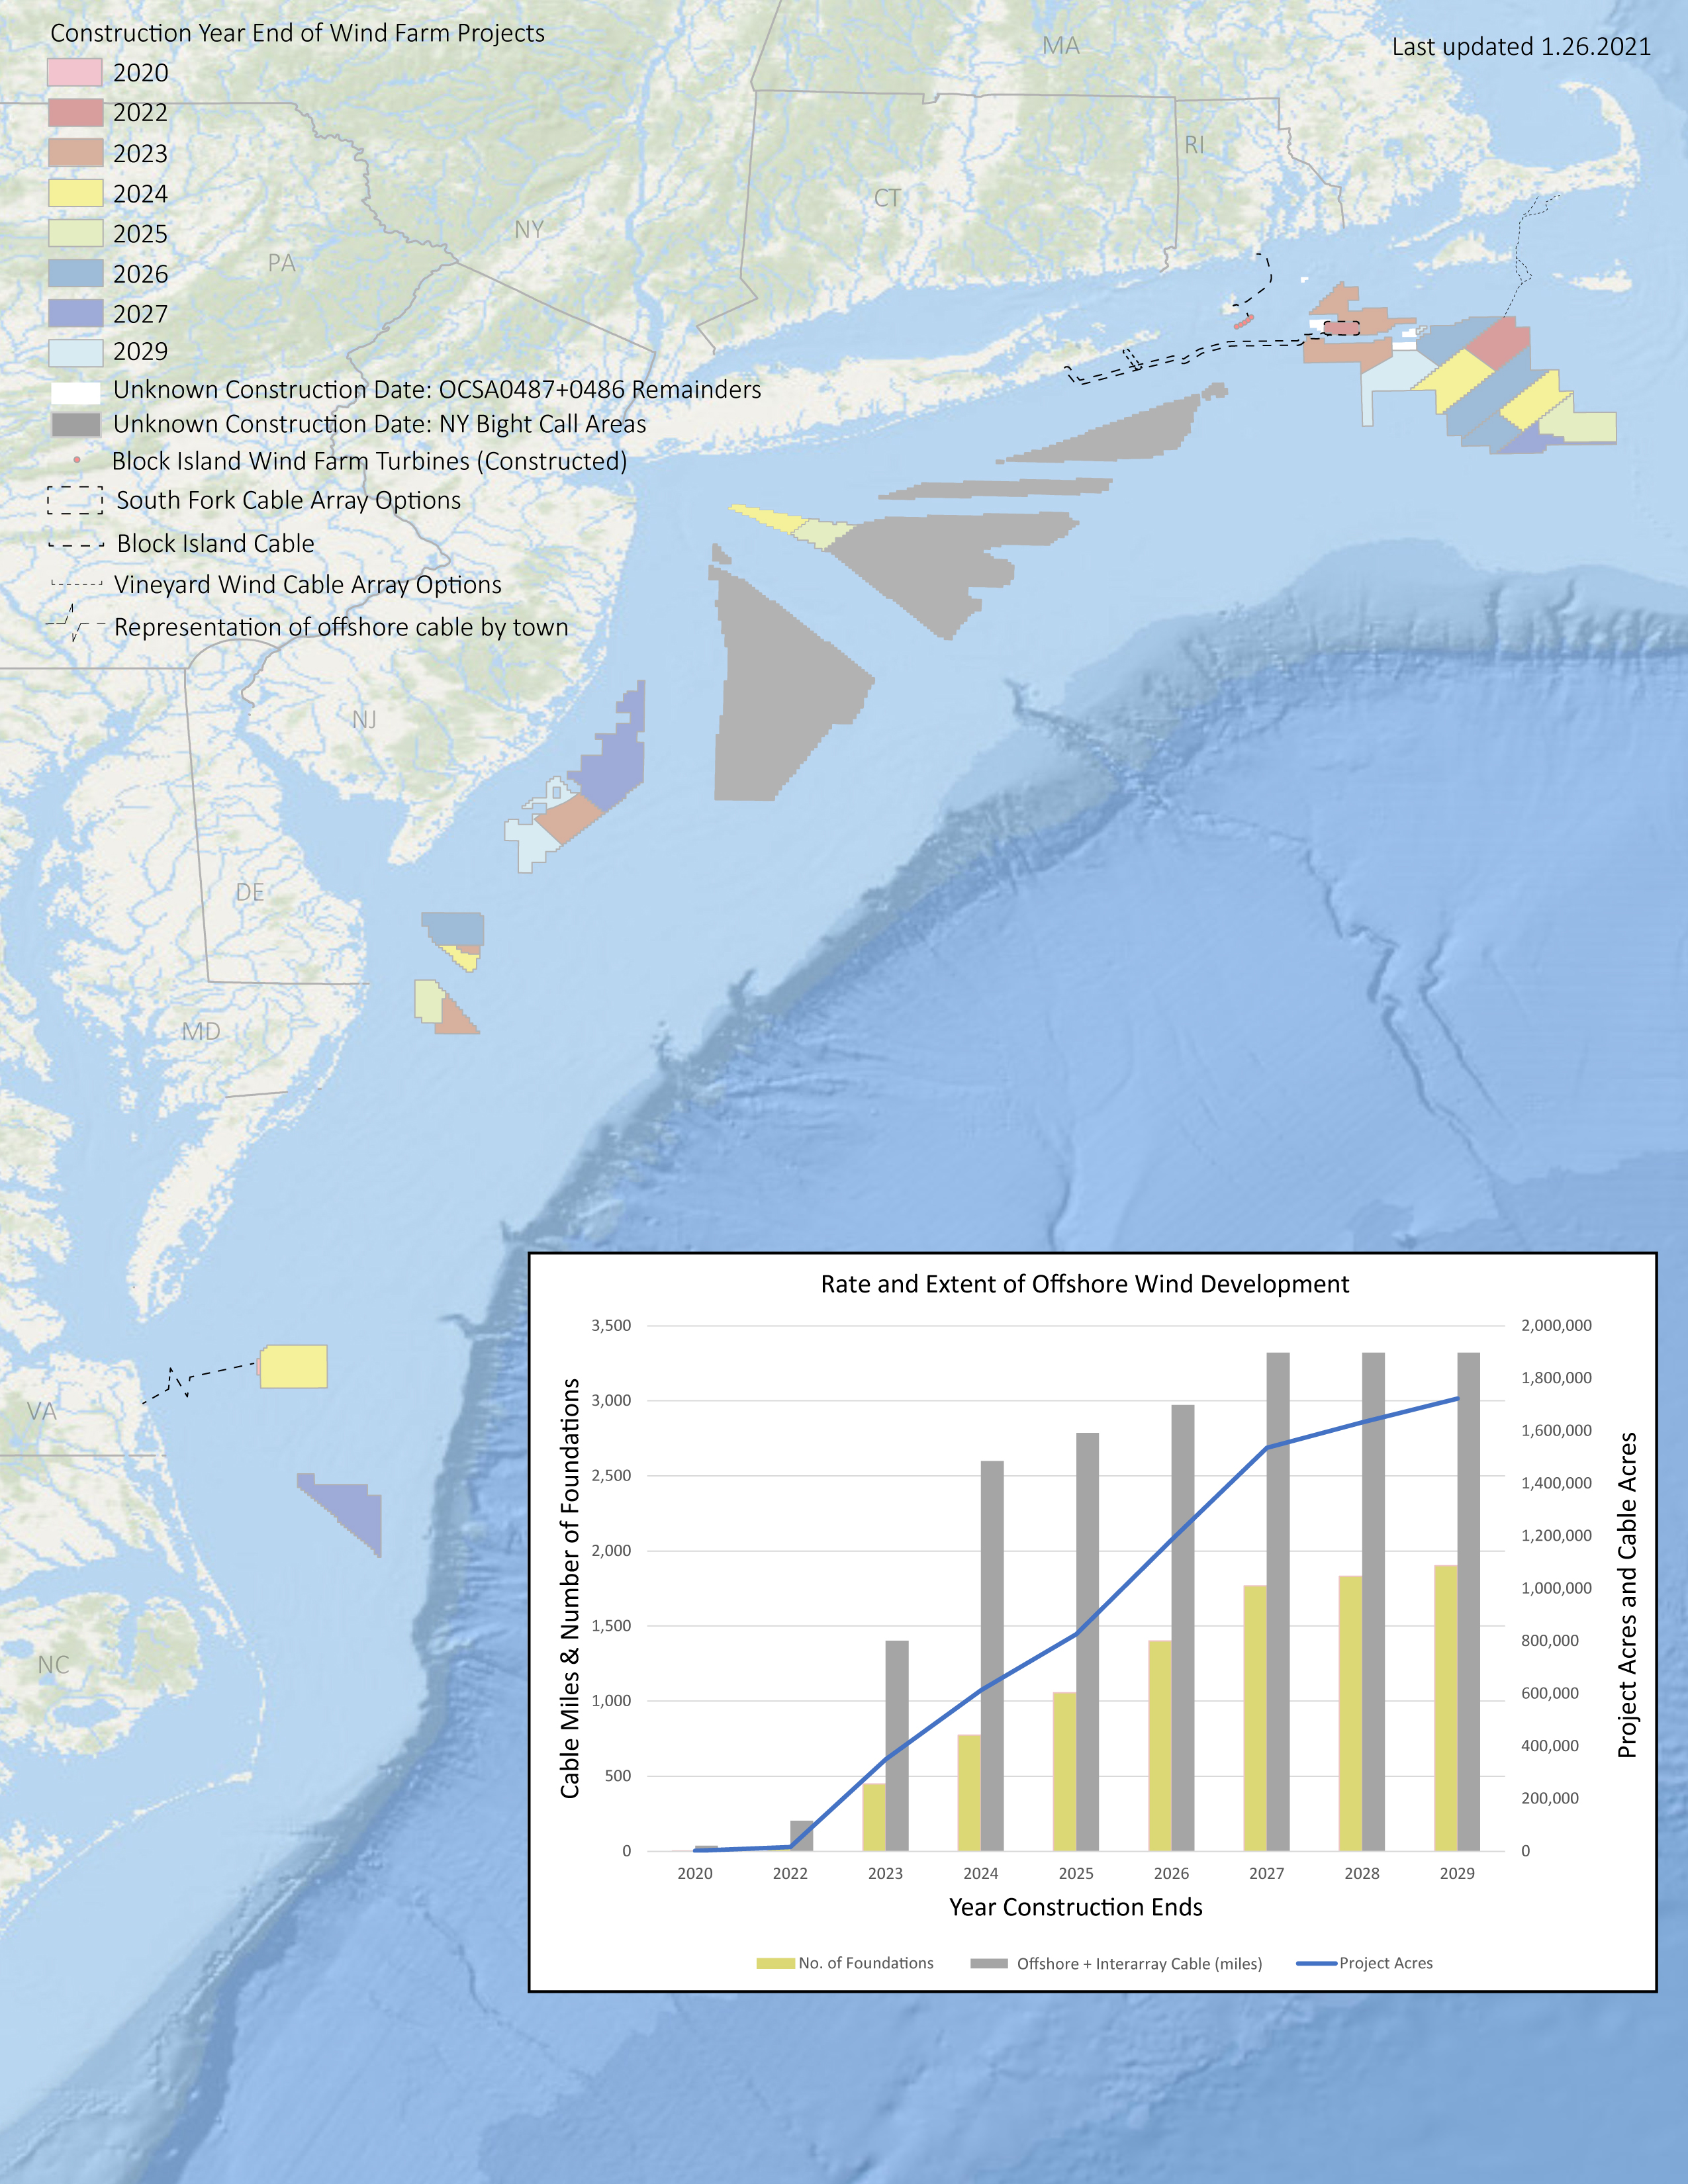
\includegraphics[width=0.9\linewidth]{images/All_2021128_needsgraph-01} 

}

\caption{All Northeast Project areas by year construction ends (each project has 2 year construction period). Data for cumulative project areas, number of foundations, offshore cable area (acres) and offshore cable and interarray cable (mile) are displayed in the graph.}\label{fig:wind-dev-cumul}
\end{figure}

Based on vessel logbook data, average commercial fishery revenue from
trips in the proposed offshore wind lease areas and the New York Bight
Call Areas represented 2-24\% of the total average revenue for each
MAFMC managed fishery from 2008-2018 (Fig. \ref{fig:wind-revenue}).

The surfclam/ocean quahog fishery was the most affected fishery, with a
maximum of 31\% of annual fishery revenue occurring within potential
wind lease areas during this period. The golden and blueline tilefish
fisheries and spiny dogfish fishery were the least affected, at 3-4\%
maximum annual revenue affected, respectively. A maximum of 11\% of the
annual monkfish revenues were affected by these areas, with similar
effects for the bluefish (10\%), summer flounder/scup/black sea bass
(9\%), and mackerel/squid/butterfish (8\%) fisheries. The New York Bight
Call Areas represented only 1-5\% of total average fishery revenue from
any fishery during 2008-2018, with the surfclam/ocean quahog fishery
most affected.

\begin{figure}

{\centering \includegraphics{SOE-MAFMC-2021_files/figure-latex/wind-revenue-1} 

}

\caption{Wind energy revenue in the Mid-Atlantic}\label{fig:wind-revenue}
\end{figure}

Proposed wind energy project areas and NY Bight Call Areas interact with
the region's federal scientific surveys (Fig.
\ref{fig:wind-dev-survey}). The total survey area overlap ranges from
1-14\% across ecosystem, shellfish, fish, shark, and protected species
surveys. For example, the sea scallop survey will have significant
overlap (up to 96\% of individual strata) while the bottom trawl survey
will have up to 60\% overlap. Additionally, up to 50\% of the southern
New England North Atlantic right whale survey's area overlaps with
proposed project areas.

\begin{figure}

{\centering \includegraphics[width=0.8\linewidth]{images/SurveyMap2021210_renamed} 

}

\caption{Interaction of Greater Atlantic Fisheries Scientific Surveys and Offshore Wind Development}\label{fig:wind-dev-survey}
\end{figure}

\hypertarget{implications-7}{%
\subsubsection{Implications}\label{implications-7}}

Current plans for rapid buildout of offshore wind in a patchwork of
areas spreads the impacts differentially throughout the region (Fig.
\ref{fig:wind-dev-cumul-MAB}).\\

\begin{figure}

{\centering \includegraphics[width=0.7\linewidth]{images/MidAtlantic_2021128-01 (1)} 

}

\caption{Zoomed in areas with name of Project, number of foundations within each project area and the states that have declared power purchase agreements.}\label{fig:wind-dev-cumul-MAB}
\end{figure}

2-24\% of total average revenue for major Mid-Atlantic commerical
species in lease areas could be displaced if all sites are developed.
Displaced fishing effort can alter fishing methods, which can in turn
change habitat, species (managed and protected), and fleet interactions.

Right whales may be displaced, and altered local oceanography could
affect distribution of their zooplankton prey.

Scientific data collection surveys for ocean and ecosystem conditions,
fish, and protected species will be altered, potentially increasing
uncertainty for management decision making.

\hypertarget{contributors}{%
\section{Contributors}\label{contributors}}

\textbf{Editors} (NOAA NMFS Northeast Fisheries Science Center, NEFSC):
Sarah Gaichas, Kimberly Bastille, Geret DePiper, Kimberly Hyde, Scott
Large, Sean Lucey, Chris Orphanides

\textbf{Contributors} (NEFSC unless otherwise noted): Andy Beet, Ruth
Boettcher (Virginia Department of Game and Inland Fisheries), Mandy
Bromilow and CJ Pellerin (NOAA Chesapeake Bay Office), Joseph Caracappa,
Doug Christel (GARFO), Patricia Clay, Lisa Colburn, Jennifer Cudney and
Tobey Curtis (NMFS Atlantic HMS Management Division), Geret DePiper,
Emily Farr and Grace Roskar (NMFS Office of Habitat Conservation),
Michael Fogarty, Paula Fratantoni, Kevin Friedland, Sarah Gaichas, Ben
Galuardi (GAFRO), Avijit Gangopadhyay (School for Marine Science and
Technology, University of Massachusetts Dartmouth), James Gartland
(Virginia Institute of Marine Science), Glen Gawarkiewicz (Woods Hole
Oceanographic Institution), Sean Hardison, Kimberly Hyde, John Kosik,
Steve Kress and Don Lyons (National Audubon Society's Seabird
Restoration Program), Young-Oh Kwon and Zhuomin Chen (Woods Hole
Oceanographic Institution), Andrew Lipsky, Sean Lucey, Chris Melrose,
Shannon Meseck, Ryan Morse, Kimberly Murray, Chris Orphanides, Richard
Pace, Charles Perretti, Grace Saba and Emily Slesinger (Rutgers
University), Vincent Saba, Chris Schillaci (GARFO), Angela Silva, Laurel
Smith, Talya ten Brink (GARFO), Bruce Vogt (NOAA Chesapeake Bay Office),
Ron Vogel (University of Maryland Cooperative Institute for Satellite
Earth System Studies and NOAA/NESDIS Center for Satellite Applications
and Research), John Walden, Harvey Walsh, Changhua Weng, Mark Wuenschel

\newpage

\hypertarget{document-orientation}{%
\section{Document Orientation}\label{document-orientation}}

The figure format is illustrated in Fig \ref{fig:docformat}a. Trend
lines are shown when slope is significantly different from 0 at the p
\textless{} 0.05 level. An orange line signifies an overall positive
trend, and purple signifies a negative trend. To minimize bias
introduced by small sample size, no trend is fit for \textless{} 30 year
time series. Dashed lines represent mean values of time series unless
the indicator is an anomaly, in which case the dashed line is equal to
0. Shaded regions indicate the past ten years. If there are no new data
for 2018, the shaded region will still cover this time period. The
spatial scale of indicators is either coastwide, Mid-Atlantic states
(New York, New Jersey, Delaware, Maryland, Virginia, North Carolina), or
at the Mid-Atlantic Bight (MAB) Ecosystem Production Unit (EPU, Fig.
\ref{fig:docformat}b) level.

\begin{figure}

{\centering \includegraphics{SOE-MAFMC-2021_files/figure-latex/docformat-1} 

}

\caption{Document orientation. a. Key to figures. b.The Northeast Large Marine Ecosystem.}\label{fig:docformat}
\end{figure}

Fish and invertebrates are aggregated into similar feeding categories
(Table \ref{tab:species-groupings}) to evaluate ecosystem level trends
in predators and prey.

\begin{table}[!h]

\caption{\label{tab:species-groupings}Feeding guilds and management bodies.}
\centering
\resizebox{\linewidth}{!}{
\fontsize{10}{12}\selectfont
\begin{tabular}[t]{>{\raggedright\arraybackslash}p{2cm}>{\raggedright\arraybackslash}p{4cm}>{\raggedright\arraybackslash}p{2cm}>{\raggedright\arraybackslash}p{5cm}>{\raggedright\arraybackslash}p{6cm}}
\toprule
\textbf{Guild} & \textbf{MAFMC} & \textbf{Joint} & \textbf{NEFMC} & \textbf{State or Other}\\
\midrule
Apex Predator & NA & NA & NA & bluefin tuna, shark uncl, swordfish, yellowfin tuna\\
\cmidrule{1-5}
Piscivore & bluefish, longfin squid, northern shortfin squid, summer flounder & goosefish, spiny dogfish & acadian redfish, atlantic cod, atlantic halibut, clearnose skate, little skate, offshore hake, pollock, red hake, silver hake, smooth skate, thorny skate, white hake, winter skate & fourspot flounder, john dory, sea raven, striped bass, weakfish, windowpane\\
\cmidrule{1-5}
Planktivore & atlantic mackerel, butterfish & NA & atlantic herring & alewife, american shad, blackbelly rosefish, blueback herring, cusk, longhorn sculpin, lumpfish, menhaden, northern sand lance, northern searobin, sculpin uncl\\
\cmidrule{1-5}
Benthivore & black sea bass, scup, tilefish & NA & american plaice, barndoor skate, crab,red deepsea, haddock, ocean pout, rosette skate, winter flounder, witch flounder, yellowtail flounder & american lobster, atlantic wolffish, blue crab, cancer crab uncl, chain dogfish, cunner, jonah crab, lady crab, smooth dogfish, spider crab uncl, squid cuttlefish and octopod uncl, striped searobin, tautog\\
\cmidrule{1-5}
Benthos & atlantic surfclam, ocean quahog & NA & sea scallop & blue mussel, channeled whelk, sea cucumber, sea urchin and sand dollar uncl, sea urchins, snails(conchs)\\
\bottomrule
\end{tabular}}
\end{table}

\newpage

\hypertarget{references}{%
\section*{References}\label{references}}
\addcontentsline{toc}{section}{References}

\hypertarget{refs}{}
\leavevmode\hypertarget{ref-link_global_2019}{}%
1. Link JS, Watson RA. Global ecosystem overfishing: Clear delineation
within real limits to production. Science Advances. 2019;5: eaav0474.
doi:\href{https://doi.org/10.1126/sciadv.aav0474}{10.1126/sciadv.aav0474}

\leavevmode\hypertarget{ref-gaichas_implementing_2018}{}%
2. Gaichas SK, DePiper GS, Seagraves RJ, Muffley BW, Sabo M, Colburn LL,
et al. Implementing Ecosystem Approaches to Fishery Management: Risk
Assessment in the US Mid-Atlantic. Frontiers in Marine Science. 2018;5.
doi:\href{https://doi.org/10.3389/fmars.2018.00442}{10.3389/fmars.2018.00442}

\leavevmode\hypertarget{ref-friedland_changes_2020}{}%
3. Friedland KD, Langan JA, Large SI, Selden RL, Link JS, Watson RA, et
al. Changes in higher trophic level productivity, diversity and niche
space in a rapidly warming continental shelf ecosystem. Science of The
Total Environment. 2020;704: 135270.
doi:\href{https://doi.org/10.1016/j.scitotenv.2019.135270}{10.1016/j.scitotenv.2019.135270}

\leavevmode\hypertarget{ref-pace_cryptic_2021}{}%
4. Pace RM, Williams R, Kraus SD, Knowlton AR, Pettis HM. Cryptic
mortality of North Atlantic right whales. Conservation Science and
Practice. 2021;n/a: e346.
doi:\href{https://doi.org/https://doi.org/10.1111/csp2.346}{https://doi.org/10.1111/csp2.346}

\leavevmode\hypertarget{ref-wood_rates_2020}{}%
5. Wood SA, Murray KT, Josephson E, Gilbert J. Rates of increase in gray
seal (Halichoerus grypus atlantica) pupping at recolonized sites in the
United States, 1988--2019. Swanson B, editor. Journal of Mammalogy.
2020;101: 121--128.
doi:\href{https://doi.org/10.1093/jmammal/gyz184}{10.1093/jmammal/gyz184}

\leavevmode\hypertarget{ref-hayes_north_2018}{}%
6. Hayes S, Gardner S, Garrison LP, Henry A, Leandro L. North Atlantic
Right Whales-Evaluating Their Recovery Challenges in 2018. NOAA Tech
Memo NMFS NEFSC 247. 2018.

\leavevmode\hypertarget{ref-record_rapid_2019}{}%
7. Record N, Runge J, Pendleton D, Balch W, Davies K, Pershing A, et al.
Rapid Climate-Driven Circulation Changes Threaten Conservation of
Endangered North Atlantic Right Whales. Oceanography. 2019;32.
doi:\href{https://doi.org/10.5670/oceanog.2019.201}{10.5670/oceanog.2019.201}

\leavevmode\hypertarget{ref-sorochan_north_2019}{}%
8. Sorochan KA, Plourde S, Morse R, Pepin P, Runge J, Thompson C, et al.
North Atlantic right whale (Eubalaena glacialis) and its food: (II)
interannual variations in biomass of Calanus spp. On western North
Atlantic shelves. Journal of Plankton Research. 2019;41: 687--708.
doi:\href{https://doi.org/10.1093/plankt/fbz044}{10.1093/plankt/fbz044}

\leavevmode\hypertarget{ref-zhang_role_2007}{}%
9. Zhang R, Vallis GK. The Role of Bottom Vortex Stretching on the Path
of the North Atlantic Western Boundary Current and on the Northern
Recirculation Gyre. Journal of Physical Oceanography. 2007;37:
2053--2080.
doi:\href{https://doi.org/10.1175/JPO3102.1}{10.1175/JPO3102.1}

\leavevmode\hypertarget{ref-goddard_extreme_2015}{}%
10. Goddard PB, Yin J, Griffies SM, Zhang S. An extreme event of
sea-level rise along the Northeast coast of North America in 2009--2010.
Nature Communications. 2015;6.
doi:\href{https://doi.org/10.1038/ncomms7346}{10.1038/ncomms7346}

\leavevmode\hypertarget{ref-hobday_hierarchical_2016}{}%
11. Hobday AJ, Alexander LV, Perkins SE, Smale DA, Straub SC, Oliver
ECJ, et al. A hierarchical approach to defining marine heatwaves.
Progress in Oceanography. 2016;141: 227--238.
doi:\href{https://doi.org/10.1016/j.pocean.2015.12.014}{10.1016/j.pocean.2015.12.014}

\leavevmode\hypertarget{ref-lentz_seasonal_2017}{}%
12. Lentz SJ. Seasonal warming of the Middle Atlantic Bight Cold Pool.
Journal of Geophysical Research: Oceans. 2017;122: 941--954.
doi:\href{https://doi.org/10.1002/2016JC012201}{10.1002/2016JC012201}

\leavevmode\hypertarget{ref-miller_state-space_2016}{}%
13. Miller TJ, Hare JA, Alade LA. A state-space approach to
incorporating environmental effects on recruitment in an age-structured
assessment model with an application to southern New England yellowtail
flounder. Canadian Journal of Fisheries and Aquatic Sciences. 2016;73:
1261--1270.
doi:\href{https://doi.org/10.1139/cjfas-2015-0339}{10.1139/cjfas-2015-0339}

\leavevmode\hypertarget{ref-wrightfairbanks_autonomous_2020}{}%
14. Wright‐Fairbanks EK, Miles TN, Cai W-J, Chen B, Saba GK. Autonomous
Observation of Seasonal Carbonate Chemistry Dynamics in the Mid-Atlantic
Bight. Journal of Geophysical Research: Oceans. 2020;125: e2020JC016505.
doi:\href{https://doi.org/https://doi.org/10.1029/2020JC016505}{https://doi.org/10.1029/2020JC016505}

\leavevmode\hypertarget{ref-steimle_energy_1985}{}%
15. Steimle F, Terranova R. Energy Equivalents of Marine Organisms from
the Continental Shelf of the Temperate Northwest Atlantic. Journal of
Northwest Atlantic Fishery Science. 1985;6.
doi:\href{https://doi.org/10.2960/J.v6.a11}{10.2960/J.v6.a11}

\leavevmode\hypertarget{ref-lawson_important_1998}{}%
16. Lawson JW, Magalhães AM, Miller EH. Important prey species of marine
vertebrate predators in the northwest Atlantic: Proximate composition
and energy density. Marine Ecology Progress Series. 1998;164: 13--20.
Available: \url{https://www.jstor.org/stable/24825521}

\leavevmode\hypertarget{ref-le_cren_length-weight_1951}{}%
17. Le Cren ED. The Length-Weight Relationship and Seasonal Cycle in
Gonad Weight and Condition in the Perch (Perca fluviatilis). Journal of
Animal Ecology. 1951;20: 201--219.
doi:\href{https://doi.org/10.2307/1540}{10.2307/1540}

\leavevmode\hypertarget{ref-millette_water_2020}{}%
18. Millette NC, Pierson JJ, North EW. Water temperature during winter
may control striped bass recruitment during spring by affecting the
development time of copepod nauplii. ICES Journal of Marine Science.
2020;77: 300--314.
doi:\href{https://doi.org/10.1093/icesjms/fsz203}{10.1093/icesjms/fsz203}

\leavevmode\hypertarget{ref-martino_recruitment_2010}{}%
19. Martino EJ, Houde ED. Recruitment of striped bass in Chesapeake
Bay:: Spatial and temporal environmental variability and availability of
zooplankton prey. Marine Ecology Progress Series. 2010;409: 213--228.
Available: \url{https://www.jstor.org/stable/24873989}

\leavevmode\hypertarget{ref-north_linking_2003}{}%
20. North E, Houde E. Linking ETM physics, zooplankton prey, and fish
early-life histories to striped bass Morone saxatilis and white perch M.
Americana recruitment. Marine Ecology Progress Series. 2003;260:
219--236.
doi:\href{https://doi.org/10.3354/meps260219}{10.3354/meps260219}

\leavevmode\hypertarget{ref-bauer_temperature-_2010}{}%
21. Bauer LJ, Miller TJ. Temperature-, Salinity-, and Size-Dependent
Winter Mortality of Juvenile Blue Crabs ( Callinectes sapidus ).
Estuaries and Coasts. 2010;33: 668--677. Available:
\url{https://www.jstor.org/stable/40663676}

\leavevmode\hypertarget{ref-hines_predicting_2011}{}%
22. Hines AH, Johnson EG, Darnell MZ, Rittschof D, Miller TJ, Bauer LJ,
et al. Predicting Effects of Climate Change on Blue Crabs in Chesapeake
Bay. Biology and Management of Exploited Crab Populations under Climate
Change. Alaska Sea Grant, University of Alaska Fairbanks; 2011. pp.
109--127.
doi:\href{https://doi.org/10.4027/bmecpcc.2010.22}{10.4027/bmecpcc.2010.22}

\leavevmode\hypertarget{ref-rome_linking_2005}{}%
23. Rome MS, Young-Williams AC, Davis GR, Hines AH. Linking temperature
and salinity tolerance to winter mortality of Chesapeake Bay blue crabs
(Callinectes sapidus). Journal of Experimental Marine Biology and
Ecology. 2005;319: 129--145.
doi:\href{https://doi.org/10.1016/j.jembe.2004.06.014}{10.1016/j.jembe.2004.06.014}

\leavevmode\hypertarget{ref-kimmel_relationship_2014}{}%
24. Kimmel DG, Tarnowski M, Newell RIE. The Relationship between
Interannual Climate Variability and Juvenile Eastern Oyster Abundance at
a Regional Scale in Chesapeake Bay. North American Journal of Fisheries
Management. 2014;34: 1--15.
doi:\href{https://doi.org/10.1080/02755947.2013.830999}{10.1080/02755947.2013.830999}

\leavevmode\hypertarget{ref-pousse_energetic_2020}{}%
25. Pousse E, Poach ME, Redman DH, Sennefelder G, White LE, Lindsay JM,
et al. Energetic response of Atlantic surfclam Spisula solidissima to
ocean acidification. Marine Pollution Bulletin. 2020;161: 111740.
doi:\href{https://doi.org/10.1016/j.marpolbul.2020.111740}{10.1016/j.marpolbul.2020.111740}

\leavevmode\hypertarget{ref-thomsen_moderate_2010}{}%
26. Thomsen J, Melzner F. Moderate seawater acidification does not
elicit long-term metabolic depression in the blue mussel Mytilus edulis.
Marine Biology. 2010;157: 2667--2676.
doi:\href{https://doi.org/10.1007/s00227-010-1527-0}{10.1007/s00227-010-1527-0}

\leavevmode\hypertarget{ref-lannig_impact_2010}{}%
27. Lannig G, Eilers S, Pörtner HO, Sokolova IM, Bock C. Impact of Ocean
Acidification on Energy Metabolism of Oyster, Crassostrea
gigas---Changes in Metabolic Pathways and Thermal Response. Marine
Drugs. 2010;8: 2318--2339.
doi:\href{https://doi.org/10.3390/md8082318}{10.3390/md8082318}

\leavevmode\hypertarget{ref-mills_fisheries_2013}{}%
28. Mills K, Pershing A, Brown C, Chen Y, Chiang F-S, Holland D, et al.
Fisheries Management in a Changing Climate: Lessons From the 2012 Ocean
Heat Wave in the Northwest Atlantic. Oceanography. 2013;26.
doi:\href{https://doi.org/10.5670/oceanog.2013.27}{10.5670/oceanog.2013.27}

\leavevmode\hypertarget{ref-boem_bureau_2021}{}%
29. BOEM. Bureau of Ocean Energy Management (BOEM). South Fork Wind Farm
and South Fork Export Cable Project Draft Environmental Impact
Statement. OCS EIS/EA BOEM 2020-057. {[}Internet{]}. 2021. Available:
\url{https://www.boem.gov/sites/default/files/documents/renewable-energy/SFWF-DEIS_0.pdf}

\end{document}
